\documentclass[12pt, a4paper]{report}
\usepackage[ngerman]{babel}
\usepackage{listings}
\usepackage{graphicx}
\usepackage{subcaption}
\usepackage[table]{xcolor}
\graphicspath{ {assets/images/} }
\usepackage{titling}
\usepackage{tabularx}
\usepackage{caption}
\usepackage{datetime}
\newdateformat{gerFormat}{\THEDAY. \monthname[\THEMONTH] \THEYEAR}
\usepackage{minted}
\usepackage{hyperref}
\graphicspath{{assets/images/}}
\usepackage[backend=biber]{biblatex}
\addbibresource{literature/moritz.bib}
\setminted[python]{tabsize=2, linenos, breakanywhere, breaklines, frame=lines, fontsize=\footnotesize}
\usepackage{setspace}
\onehalfspacing % Setze Zeilenabstand auf 1,5-fach
\begin{document}
\pagenumbering{roman}
%TITLING
\pretitle{%	
	\begin{center}
	\LARGE
	
\includegraphics[scale=1]{DHBW.jpg}\\[\bigskipamount]
}
\posttitle{
	\end{center}
}
\preauthor{%
	\begin{center}
	\vspace{1cm}	
	im Studiengang Cybersecurity\\
	\vspace{1cm}	
	an der Dualen Hochschule Baden-Württemberg Mannheim\\
	\vspace{1cm}
	von
	
}
\postauthor{
	\vspace{1cm}
	\end{center}
	\begin{minipage}{\textwidth}
        \begin{center}
            Jonas Grohe,\\
            Steven Hartinger,\\
            Moritz Reufsteck            
        \end{center}
	\end{minipage}
    \vspace{1cm}
    \begin{center}
        Bearbeitungszeitraum: 18.01.2022 - 01.09.2022\\
        Fachlicher Betreuer: Prof. Dr. Holger Hofmann
    \end{center}
}

\begin{titlepage}
    \title{Mobile Schwarmintelligenz: Navigation eines Raspberry Pi Roboters mittels Schwarmintelligenz}
    % add a title description

    %\author{Moritz Reufsteck}
    %\date{\gerFormat\today}
    \date{\vspace{-5ex}}
    %\date{}  % Toggle commenting to test  
    \maketitle
\end{titlepage}
<<<<<<< HEAD
\chapter{Schwarmintelligenzalgorithmen}
\section{Partikelschwarmoptimierung}
Die Partikelschwarmoptimierung/particle swarm optimization (PSO) wurde zuerst von Dr. Kennedy und Dr. Eberhart in 1995 vorgestellt.
 Sie ist inspiriert vom Verhalten von Vogelschwärmen und Fischschulen. Jeder Teil wird als Partikel bezeichnet, die Gesamtheit als Schwarm.
\\ Die Partikel werden gleichverteilt über dem Suchbereich verteilt. Sie erhalten eine zufällige Startgeschwindigkeit. 
Der Suchraum hat \textbf{D} Dimensionen und \textbf{N} ist die Menge an Partikeln. Nun hat das \textbf{i}-te Partikel die Position X\textsubscript{i}=(x\textsubscript{i1},x\textsubscript{i2},x\textsubscript{i3},... ...,x\textsubscript{iD})
  und die Geschwindigkeit V\textsubscript{i}(v\textsubscript{i1},v\textsubscript{i2},v\textsubscript{i3},... ...,v\textsubscript{iD}). Außerdem speichert jedes Partikel seine beste Position P\textsubscript{ibest} und erhält die insgesamt beste Position P\textsubscript{gbest}. 
\\
Jedes Partikel updated seine Position nach den folgenden Gleichungen:\\
V\textsubscript{i}\textsuperscript{K+1}=wV\textsubscript{i}\textsuperscript{K}+c\textsubscript{1}r\textsubscript{1}(P\textsubscript{ibest}-X\textsubscript{i}\textsuperscript{K})+c\textsubscript{2}r\textsubscript{2}(P\textsubscript{gbest}-X\textsubscript{i}\textsuperscript{K})\\
$X_i^{K+1}=X_i^K+V_i^{K+1}$
\begin{itemize}

  \item k: Nummer der Iteration
  \item i: Nummer des Partikels
  \item w: Startgewicht, gibt an wie stark/schwach sich die Geschwinidgkeit pro Iteration verändert, um Divergenz zu vermeiden sollte es  kleiner als 1 gewählt werden
  \item c1,c2: kognitives und soziales Gewicht, positive Konstanten

\end{itemize}
Schritte der gründsätzlichen Durchführung der Partikelschwarmoptimierung:
\begin{enumerate}
  \item Initialisierung: Die Partikel werden gleichverteilt initialisiert und erhalten eine Startgeschwindigkeit
  \item Evaluierung: Die Partikel werden nach einer Fitnessevaluierung ausgewertet 
  \item Update P: Der so gewonnene Fitnesswert wird dem bisher besten Fitnesswert des Partikels verglichen, ist er besser wird $P_{ibest}=P_i$. Ist dieser Wert auch besser als $P_{gbest}$ so ersetzt $P_i P_{gbest}$
  \item Update Partikel: Die Position und Geschwindigkeit werden nach den obigen Formeln verändert.
  \item Wiederholung: Schritt 2 bis 4 werden nun bis Erreichen des Abbruchkriteriums wiederholt
\end{enumerate}\\

Hier gibt es nun noch verschieden Einflüsse auf die Umsetzung der Partikelschwarmoptimierung.
Das Abbruchkriterium kann unterschiedlich gewählt werden. Standardmäßig werden hier entweder die Anzahl der Iterationen im Vorhinein festgelegt oder der Algorithmus endet nach einer zu geringen Änderung nach mehreren Iterationen. 
Um die Konvergenz zu beschleunigen kann der $P_{ibest}$-Wert anstatt des persönlich besten Wertes den besten Wert eines bestimmten Umfelds speichern.
Der Wahl der Fitnessevaluierung muss hier ein großer Wert zukommen. Eine gut gewählte Fitnessfunktion kann die Konvergenz stark beschleunigen und somit den benötigten Rechenaufwand minimieren.\\
PSO teilt viele Merkmale mit genetischen Algorithmen. Beide basieren auf einer zufälligen Initialisierung ihrer Agenten und entwickeln diese Anhand einer Fitnessevaluierung weiter. Allerdings erfolgt der Informationsaustausch grundlegend unterschiedlich. Während bei einem genetischen Algorithmus alle Agenten untereinander Informationen austauschen, erfolgt dies bei einer PSO nur in eine Richtung, vom besten Partikel zu allen anderen.\\


\begin{figure}
  \centering
  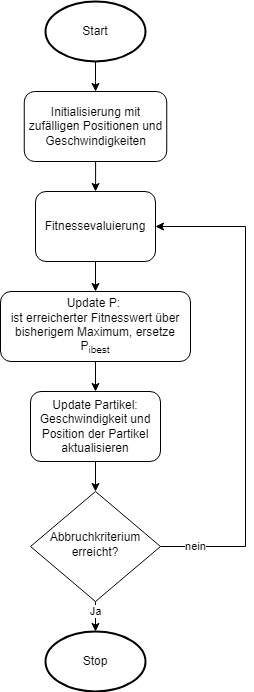
\includegraphics[scale=0.75]{Flow_PSO.png}
  \caption{Flussdiagramm von PSO}
  \label{fig:Figure_PSO}
\end{figure}


\section{Ameisen Algorithmen}
Ameisenalgorithmuen sind von der Futtersuche der Ameisen abgeleitet. Jede Ameise scheidet auf ihrem Weg Pheromone aus, welche mit der Zeit verdunsten. 
Folgende Ameisen wählen wahrscheinlicher einen Weg mit größerer Pheromonkonzentration. 
Existieren nun zwei unterschiedlich lange Wege mit gleicher Pheromonkonzentration, entscheiden sich etwa gleich viele Ameisen für beide Wege. 
Da die Ameisen auf dem kürzeren Weg in gleicher Zeit allerdings öfter laufen, steigt hier die Konzentration schneller als auf dem längeren Weg. 
Infolgedessen laufen immer mehr Ameisen den kürzeren Weg und es bildet sich eine Ameisenstraße.\\

Es gibt viele verschiedene Umsetzungen der Ameisenalgorithmen. Der erste Ansatz wurde von Marco Dorigo 1991 vorgestellt\cite{Dorigo1991AntSA} und 1996 nochmal verbessert\cite{484436}.
Sein Ansatz namens \emph{Ant System} lieferte Grundlagen welche er 1997 in einem neuen System namens \emph{Ant Colony System} weiter verbesserte\cite{585892}.\\
Schließlich veröffentlichte er in 2006 die \emph{Ant Colony Optimization (ACO)} welche im folgenden vorgestellt wird\cite{4129846} \\

Jede Ameise bewegt sich von Punkt x zu Punkt y mit folgender Wahrscheinlichkeit:\\
\large$p_{xy}^k=\frac{(T_{xy}^a)(n_{xy}^b)}{\Sigma(T_{xy}^a)(n_{xy}^b) }$

\begin{itemize}
  \item $T_x_y$: Menge an Pheromonen auf dem Übergang von x nach y 
  \item a: Gewicht des Einflusses von $T_x_y$
  \item $n_x_y$: Maß wie wünschenswert dieser Übergang ist, wird häufig aus Abstand zum Ziel berechnet
  \item b: Gewicht des Einflusses von $n_x_y$
\end{itemize}

Nun bewegt sich jeder Agent nach der von ihm berechneten Wahrscheinlichkeit, bis er den Zielzustand erreicht. Dann werden die Pheromone folgendermaßen aktualisiert:\\
$T_x_y^k=(1-p)T_x_y^k+\Delta T_x_y^k$
\begin{itemize}
  \item p: Pheromonverdunstung
  \item \delta $T_x_y$: in diesem Schritt ausgeschüttete Pheromone
\end{itemize}
Schritte der grundsätzlichen Durchführung von ACO:
\begin{enumerate}
  \item Initialisierung: Die Übergänge zwischen Start und Ziel bekommen einen Wert für n zugewiesen
  \item Jede Einheit bewegt sich einen Schritt übereinstimmend mit der berechneten Wahrscheinlichkeit.  Wiederholen, bis das Ziel erreicht ist
  \item Die Länge der Pfade messen und Pheromonkonzentration aktualisieren
  \item Die Länge aller Pfade mit dem bisherigen besten Pfad vergleichen, den besten Pfad speichern
  \item Wiederholung: Schritt 2-4 wiederholen bis Abbruchkriterium erreicht ist
\end{enumerate}

\begin{figure}
  \centering
  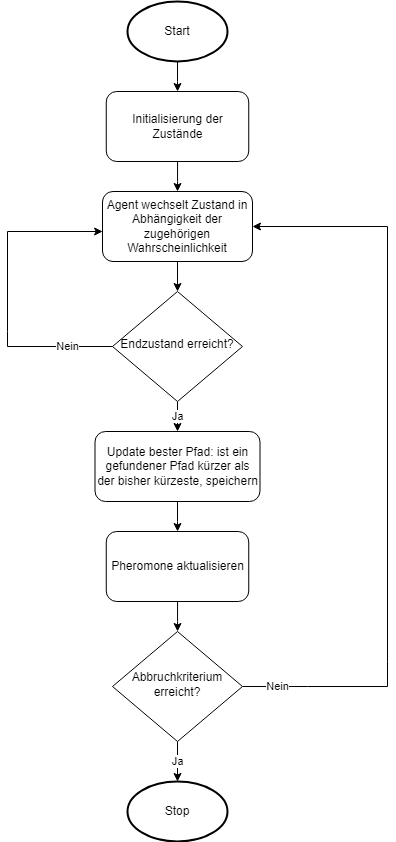
\includegraphics[scale=0.75]{Flow_ACO.png}
  \caption{Flussdiagramm von ACO}
  \label{fig:Figure_ACO}
\end{figure}

\section{Bienen Algorithmen}
Der Bienen Algorithmus ist von der Futtersuche der Bienen abgeleitet. Ein kleiner Teil des Bienenschwarms fungiert als Kundschafter für die Kolonie.
Sie sind konstant zufällig auf der Futtersuche. Finden sie eine Futterquelle analysieren sie deren Effektivität und kehren zum Bienenstock zurück. Die Effektivität hängt von Faktoren wie der Menge, Entfernung und Zuckergehalt ab.\cite{PHAM2006454}
Die Bienen, die eine effektive Futterquelle gefunden haben, führen nun einen sogenannten \emph{waggle dance} auf dem \emph{dance floor} aus \cite{Seeley+1995}. Damit gibt sie die Wegbeschreibung zur Futterquelle weiter.
Unbeschäftigte Arbeiterbienen schauen auf dem dance floor nach Wegbeschreibungen. Umso effektiver die Futterquelle, umso länger der Tanz, daher werden auch mehr Arbeiterbienen diese ausnutzen.\cite{KARABOGA2009108}\\

Im Artificial Bee Colony (ABC) Algorithmus gibt es drei Gruppen an Bienen:
\begin{enumerate}
  \item Kundschafter (Scout) Bienen: Sie fliegen zufällig auf der Futtersuche umher
  \item Betrachter Bienen: Sie stehen am dance floor und beobachten die Tänze. Sie suchen sich den besten aus und werden nun zu beschäftigten Bienen
  \item Beschäftigte Bienen: Sie fliegen zu der von ihr gewählten Futterquelle. Nachdem sie zurückgekehrt sind kommunizieren sie ihre Informationen auf dem dance floor weiter.
\end{enumerate} 

\chapter{Vergleich der Algorithmen}
Nachdem wir oben die drei Algorithmen Particel Swarm Optimization(PSO), Ant Colony Optimization(ACO) und  Artificial Bee Colony (ABC) vorgestellt haben, werden wir sie im folgenden zuerst generell und dann spezifisch für unseren Anwendungsfall vergleichen\\

\section*{Allgemeiner Vergleich}

\subsection*{Kommunikation}
Die einzelnen Agenten der Algorithmen kommunizieren auf unterschiedliche Arten. Bei den Partikeln kommuniziert nur das allgemein oder lokal beste Partikel mit den andern. 
Die Ameisen-Agenten kommunizieren nur indirekt über die von ihnen hinterlassenen Pheromone. Bei den Bienen-Agenten funktioniert die Kommunikation sehr viel direkter.
Sie führen ihren waggle dance aus und kommunizieren damit die Wegbeschreibung sowie die Effektivität der Lösung und vergleichen diese untereinander.

\subsection*{Ausgabe}
Die Daten werden bei der PSO als beste lokale oder globale Position der Partikel gespeichert. Diese Position repräsentiert die beste gefundene Lösung für das Problem.
Bei der ACO ist die Ausgabe in den verschiedenen Pheromonkonzentrationen auf den Pfaden. Der Pfad mit der höchsten Konzentration ist die beste gefundene Lösung.
Bei der Artificial Bee Colony ist die Lösung indirekt im Tanz der Bienen enthalten. Die effektivste, gefundene Lösung wird von der Biene repräsentiert, welche den attraktivsten Tanz hat.

\subsection*{Anwendungsgebiet}
Die Algorithmen sind aufgrund ihres Aufbaus jeweils für unterschiedliche Anwendungsgebiete besonders gut geeignet. Allerdings, können die meisten Probleme in andere Gebiete überführt werden, womit auch andere Algorithmen auf sie überführbar sind.\\
Partikel Schwarm Optimierung ist am besten für Funktionsoptimierung geeignet. Es findet effektiv lokale und globale Maxima.
Die Ant Colony Optimization ist gut für das Traveling Salesman Problem sowie das Vehicle Routing Problem geeignet. Gerade bei kleineren Problemen kann es schnell eine Lösung liefern\cite{sabet2016comparison}.
Die Artificial Bee Colony ist gut für das Trainieren eines neuronalen Netzes geeignet. Für ein großes Traveling Salesman Problem schlägt es die anderen in Performance\cite{sabet2016comparison}.





=======
% LTeX: language=de-DE
\section*{Erklärung zur Eigenleistung}
Wir versichern hiermit, dass wir unsere Studienarbeit mit dem Thema: \textit{\thetitle} selbstständig verfasst und keine anderen als die angegebenen Quellen und Hilfsmittel benutzt haben. Wir versichern zudem, dass die eingereichte elektronische Fassung mit der gedruckten Fassung übereinstimmt.

\begin{minipage}{\textwidth}
    \begin{center}
        \vspace{2.5cm}
        \parbox{6cm}{\centering Mannheim, \gerFormat\today \hrule
        \strut \centering\footnotesize Ort, Datum} \hfill\parbox{4cm}{\hrule
        \strut \centering\footnotesize Steven Hartinger}        
    \end{center}
\end{minipage}

\begin{minipage}{\textwidth}
    \begin{center}
        \vspace{1cm}
        \parbox{6cm}{\centering Mannheim, \gerFormat\today \hrule
        \strut \centering\footnotesize Ort, Datum} \hfill\parbox{4cm}{\hrule
        \strut \centering\footnotesize Jonas Grohe}        
    \end{center}
\end{minipage}

\begin{minipage}{\textwidth}
    \begin{center}
        \vspace{1cm}
        \parbox{6cm}{\centering Mannheim, \gerFormat\today \hrule
        \strut \centering\footnotesize Ort, Datum} \hfill\parbox{4cm}{\hrule
        \strut \centering\footnotesize Moritz Reufsteck}        
    \end{center}
\end{minipage}
\tableofcontents
\listoffigures
\listoftables
\listoflistings
\chapter{Einleitung}
\pagenumbering{arabic}
% LTeX: language=de-DE
\section{Problemstellung}
In der modernen Robotik gibt es immer mehr Anwendungen, in denen mehrere mobile Roboter zusammenarbeiten müssen, um eine bestimmte Aufgabe auszuführen. Ein Beispiel hierfür ist die Exploration von unbekannten Umgebungen, bei der mehrere Roboter zusammenarbeiten müssen, um eine möglichst große Fläche abzudecken. Ein wichtiger Aspekt in diesen Anwendungen ist die Fähigkeit der Roboter, effizient und koordiniert zu navigieren, um Kollisionen und unnötige Rückwege zu vermeiden. Für einen Austausch der Informationen unter den einzelnen Robotern muss eine zuverlässige Kommunikation stattfinden.
Ein Ansatz, um dieses Problem anzugehen, ist die Anwendung von Pathfinding-Algorithmen, die es den Robotern ermöglichen, einen Weg durch die Umgebung zu finden, der ihre Ziele erreicht und gleichzeitig die Ressourcen wie zum Beispiel Energie und Zeit der Roboter optimiert. In dieser Arbeit soll untersucht werden, wie Pathfinding-Algorithmen in einer Umgebung mit mehreren mobilen Robotern angewendet werden können, um eine koordinierte und effiziente Navigation zu ermöglichen. 

\section{Ziel der Arbeit}
Schwarmintelligenz beschreibt das Phänomen, dass ein Schwarm von Lebewesen oder künstlichen Agenten in der Lage ist, gemeinsam komplexe Aufgaben zu lösen, die für einzelne Individuen unlösbar wären. Schwarmintelligenz findet sich in der Natur bei vielen Arten, wie beispielsweise Ameisen, Bienen oder Schwärmen von Vögeln oder Fischen. Der Schlüssel zur Schwarmintelligenz liegt in der Fähigkeit der Individuen, miteinander zu kommunizieren und Informationen auszutauschen.
In der Technologie wird Schwarmintelligenz zunehmend genutzt, um komplexe Aufgaben zu lösen. Mobile Schwarmintelligenz beschreibt dabei den Einsatz von Schwarmintelligenz in mobilen Systemen wie beispielsweise Robotern oder Drohnen. Diese können sich eigenständig in einer Umgebung bewegen und gemeinsam Aufgaben erledigen, die für einzelne Roboter oder Drohnen zu schwierig wären.
Um Schwarmintelligenz in mobilen Systemen zu nutzen, gibt es eine Vielzahl von Algorithmen. Beispiele hierfür sind der Bienen-Algorithmus, der Ameisenalgorithmus oder der Partikel-Schwarm-Algorithmus. Diese Algorithmen nutzen unterschiedliche Strategien, um Schwarmintelligenz in mobilen Systemen zu erzeugen.
Im Rahmen dieser Arbeit soll ein geeigneter Algorithmus für die Navigation eines Einplatinencomputers durch einen Hindernisparcours mittels Schwarmintelligenz ermittelt werden. Hierfür sollen verschiedene Algorithmen vorgestellt und miteinander verglichen werden. Der ausgewählte Algorithmus soll es dem Einplatinencomputer ermöglichen, Hindernisse eines Parcours zu verarbeiten und eine optimale Route durch den Parcours zu finden.
Damit die Schwarmintelligenz-Algorithmen auf dem Einplatinencomputer ausgeführt werden können, ist eine zuverlässige Kommunikation mit einem Server notwendig. Hierfür können beispielsweise WLAN- oder Bluetooth-Verbindungen genutzt werden. Die Kommunikation muss dabei praktisch und zuverlässig umgesetzt werden, um eine fehlerfreie Navigation durch den Hindernisparcours zu gewährleisten.
Um den Einplatinencomputer für die Navigation durch den Parcours fit zu machen, muss dieser zu einem Roboter umgebaut werden. Hierfür werden geeignete Bauteile benötigt, die dem Roboter die Fähigkeit zum Fahren, Lenken und Orientieren geben. Die Bewegung des Roboters kann mithilfe von Servomotoren umgesetzt werden, die eine präzise Steuerung der Bewegungen ermöglichen.
Insgesamt zeigt sich, dass Schwarmintelligenz ein vielversprechendes Konzept für die Navigation von mobilen Systemen in komplexen Umgebungen ist. Durch die Nutzung von Schwarmintelligenz-Algorithmen können Roboter oder Drohnen eigenständig und effizient Aufgaben erledigen, die für einzelne Individuen zu schwierig wären.

\section{Vorgehensweise}
Zu Beginn der Arbeit wird der Begriff Schwarmintelligenz erläutert und in Bezug auf die Nutzung mobiler beziehungsweise beweglicher Geräte gebracht. Im folgenden Schritt werden verschiedene Pathfinding-Algorithmen erläutert und ihre Anwendbarkeit auf die vorliegende Problematik evaluiert. Daraufhin erfolgt eine genaue Beschreibung, inklusive Zielsetzung, des praktischen Anwendungsbeispiels.   
In der Planungsphase sollen Entscheidungen darüber getroffen werden, welche technischen Lösungen ausgewählt werden. Mögliche Entscheidungsfindungen sind hier beispielsweise verwendete Hardware, Bibliotheken oder Frameworks. Anschließend sollen die zuvor erlangten Kenntnisse und Entwürfe dazu genutzt werden, eine Umsetzung in Form eines Prototyps zu entwickeln.

\chapter{Schwarmintelligenz}
% LTeX: language=de-DE
\section{Ansätze aus der Natur}
In dieser Arbeit werden grundlegend drei verschiedene Algorithmen der Schwarmintelligenz für unsere Problematik  erläutert und evaluiert. Jede dieser Algorithmen sind Analogien zu dem Verhalten von Lebewesen aus der Natur. Schwarmoptimierungsalgorithmen (SOAs) imitieren die kollektive Explorationsstrategie von Schwärmen in der Natur bei Optimierungsproblemen. Diese Algorithmen verwenden einen populationsbasierten Ansatz für die Probleme. Diese Gruppe von Algorithmen wird als populationsbasierte stochastische Algorithmen bezeichnet.

Der erste Algorithmus ist der Bees Algorithm (BA). Dieser basiert auf der Nahrungssuche von Honigbienen. Honigbienen sammeln ihr Essen über mehrere Kilometer, weshalb ein organisierter Ablauf und Kommunikation die Schlüssel des Erfolges sind. Die Bienen gehen dabei so vor, dass sie sogenannte Späher-Bienen zur Nahrungsfindung aussenden. Sind diese Späher erfolgreich, kehren sie zurück zum Bienenstock und informieren die anderen Bienen per Tanz über den Standorts des Essens. Anhand dieser Information können die anderen Honigbienen das Essen sammeln, während die Späher versuchen, weitere Blumenbeete ausfindig zu machen. Quelle: Clever Algorithms

Ein weiterer relevanter Algorithmus zur Optimierung eines Schwarms ist die Particle Swarm Optimization (PSO). Dieser nutzt das Verhalten von Populationsgruppen wie beispielsweise Herdentieren oder  Vogel- bzw. Fischschwärmen. Dabei steht der Schwarm für die Population und jedes Mitglied der Population wird Partikel genannt. Die Partikel sind bei der Optimierung entscheidend, da sie das globale Optimum finden sollen. Dies erreichen, indem sie iterativ versucht, Partikel im Hinblick auf ein bestimmtes Qualitätsmaß zu verbessern. Dabei wird ein Partikel abhängig von seiner Position und Geschwindigkeit zu der besten bekannten Position geführt und informiert die anderen Partikel über seine Position. Falls nun ein anderer Partikel eine bessere Position als die vorherige gefunden hat, werden die anderen Partikel benachrichtigt und der Schwarm in die Richtung gelenkt. Dies geschieht so lange, bis der Schwarm innerhalb des Suchraumes die optimale Position gefunden hat. 

Der letzte Algorithmus, der in dieser Arbeit vorgestellt wird, ist der Ant System Algorithmus. Inspiriert ist dieser Algorithmus von der Essenssuche von Ameisen. Ameisen sind so gut wie blind weshalb sie bei der Nahrungsfindung über Pheromone kommunizieren. Schüttet eine Ameise Pheromone aus, bedeutet es, dass sie Nahrung gefunden hat. Dies geschieht jedes Mal, sobald eine Ameise Essen findet. Durch das positive Feedback wissen die Ameisen also, welcher Route sie folgen müssen. Über die Zeit verfallen die Pheromone, damit alte Pfade nicht mehr gefolgt werden. 
Clever Algorithms

\section{Mobile Schwarm Intelligenz}
Durch komplexer werdende Probleme in allen Bereichen des Lebens ist es von Relevanz, dass schnelle und effiziente Ansätze zur Lösung von Problemen gefunden werden. Besonders wenn ein Informationsaustausch oder lokale Kommunikation einer Mehrzahl von Systemen stattfindet, kann Schwarm Intelligenz (oder auch Kollektive Intelligenz genannt) bei der Lösung von Problemstellungen helfen. Als Inspiration vieler Grundlagen Schwarm-basierter Systeme dient das biologische Verhalten von Vorkommnissen in der Natur, wie das von Insekten wie beispielsweise Ameisen, oder das Verhalten von in Schwärmen agierenden Lebewesen wie Fischen oder Vögeln \cite{Blum2008}. 
Ein Schwarm, der in der Natur als kollektives Verhalten von organisierten, jedoch dezentralisierten Populationen bekannt ist \cite{Kiranyaz2013}, wird im Jahr 1999 mit der Informationstechnik von \cite{Bonabeau1999} in Zusammenhang gebracht und als Eigenschaft bezeichnet, die es individuellen Komponenten durch Interaktion ermöglicht, Aktionen durchzuführen, die nicht durch das alleinige Handeln einer einzeln agierenden Komponente umsetzbar sind. Interaktionen, wie beispielsweise das Abgeben von Pheromonspuren auf gefundenen Wegen zwischen dem Nest einer Kolonie von Ameisen, oder dem sogenannten "waggle dance" von Bienen, deren Schwärmer diesen praktizieren, wenn sie auf neue Futterquellen gestoßen sind \cite{Blum2008, Panigrahi2011}, können in Form anderer Kommunikations- oder Interaktionsverfahren im Netzwerk- oder Datenverkehr angewendet werden. Ersteres basiert darauf, dass einzelne Ameisen das abgegebene Pheromon anderer Ameisen als indirektes Kommunikationsmedium nutzen, um damit den kürzesten Weg zu einer Futterquelle zu finden \cite{Blum2008}. Die Ameisen nutzen dabei die Dichte des Pheromons, um die Richtung zu bestimmen, in die sie sich bewegen sollen. Um dieses Verhalten auf Anwendung in der Informationstechnik übertragen zu können, werden "künstliche Pheromon" Spuren geschaffen, deren Informationsgehalt dadurch genutzt werden kann, um probabilistische Entscheidungen zu treffen. Abgegeben werden diese künstlichen Spuren dann von Agenten, die die künstlichen Ameisen darstellen \cite{Gendreau2010}.

Ein bekannter Algorithmus, der in vielen wissenschaftlichen Arbeiten wie \cite{Blum2008,Parpinelli2011,Brownlee2011} thematisiert und erläutert wird, ist die Ant-Colony-Optimization (ACO). Hierbei handelt es sich um eine metaheuristische Technik im Verhalten von Ameisen. Das Ziel der Spezies ist es, den kürzesten Weg einer Kolonie bis zu einer Futterquelle zu ermitteln \cite{Parpinelli2011}. Der aus der Biologie bekannte und definierte Schwarm wird im Jahr 1999 von \cite{Bonabeau1999} als Eigenschaft bezeichnet, die es individuellen Komponenten durch Interaktion ermöglicht, Aktionen durchzuführen, die nicht durch das alleinige Handeln einer einzeln agierenden Komponente umsetzbar sind. 
Die in der Natur vorkommenden Phänomene von Schwarmintelligenz haben zudem Forscher dazu motiviert, "intelligent mutli-agent" Systeme zu entwerfen, deren Verhalten sich stark an den Vorkommnissen und Vorbildern in der Natur orientiert. Besonders Optimierungsprobleme, beispielsweise in den Bereichen des Routings von Telekommunikationsdaten, profitieren durch die Implementierung von Schwarmintelligenz Algorithmen \cite{Blum2008}. Zudem ist das Themengebiet der Robotik ebenfalls ein Anwendungsfall, für den das ursprünglich in der Natur vorkommende Phänomen als Vorbild dient. [s. 167 Blum2008]
Im Folgenden werden drei bekannte Anwendungsfelder, die als verschiedene Anwendungsfälle für Schwarmintelligenz in einer Vielzahl von Literaturwerken \cite{Blum2008,Parpinelli2011,Eberhart2001,Spears2005} erläutert werden.
Das Phänomen der Ameisen, aus dem die metaheuristische Technik ACO (Ant Colony Optimization) hervorgeht \cite{Blum2008, Panigrahi2011, Gendreau2010}, stellt eine effektive Methode dar, um Routing Probleme in Netzwerken zu lösen. Eine weit verbreitete und umfangreich erforschte Technik hierfür ist AntNet. AntNet basiert darauf, dass Agenten zu gleicher Zeit die Gegebenheiten, das heißt, Knoten und Kanten in einem Netzwerk erforschen und währenddessen die gesammelten Informationen austauschen. Wie im biologischen Vorbild findet dieser Informationsaustausch ebenfalls indirekt statt \cite{DiCaro2011}. 
Eine weitere relevante Optimierungsmethode von Problemlösungen ist die PSO (Particle Swarm Optimization), die zum ersten Mal 1995 in \cite{Kennedy1995} thematisiert wurde und ihren Ursprung wie der ACO ebenfalls an einem der Biologie zugehörigen Phänomen hatte. Hierbei handelt es sich um einen probabilistischen Algorithmus, bei dem individuelle Partikel als Teil eines Schwarms in einem Suchraum vorhanden sind. Jedes einzelne Partikel stellt eine potenzielle Lösung für das zu behandelnde Problem dar. Diese Partikel bewegen sich durchgehend durch den Suchraum. Das Ziel hierbei ist, dass eine optimale oder ausreichend gute Lösung gefunden wird. Während des gesamten Vorgangs und weiterführenden Iterationen beobachten Partikel jeweils die Positionen der anderen Partikel. Nach jeder Iteration speichert ein Partikel den besten Fitnesswert, der während einer Suche gefunden wurde  \cite{Blum2008}.
Ein weiterhin relevanter Algorithmus, der unter anderem in den Bereichen Robotik und Netzwerk Routing Anwendung findet, ist der Bees Algorithm (BA) Einer der Algorithmen basiert auf der dezentralisierten Entscheidungsfindung von Bienenschwärmen bei der Nahrungssuche. Bienen praktizieren hierbei einen Tanz, passen ihn je nach Profitabilität der Futterquelle an und locken damit andere Bienen an. Müssen Bienen zwischen zwei Kandidaten entscheiden, wählen sie diejenige, deren waggle-dance stärker ausgeprägt ist \cite{Panigrahi2011, Yuce2013, Parpinelli2011}. Ist die Futterquelle einer anderen Biene vielversprechender als die, zu der sich eine Biene zu diesem Zeitpunkt bewegt, verwirft sie die eigene und macht sich auf den Weg zu der Quelle, die die andere Biene preisgegeben hat \cite{Bonabeau1999}. Die Analyse des resultierenden Algorithmus zeigt die Existenz von zwei Typen von Bienen: Scout-Bienen und Arbeiter-Bienen. Die Arbeiter-Bienen nutzen die bereits von den Scout-Bienen gesammelten Informationen, um eine erfolgreiche Lokalisierung von Nahrungsquellen zu erreichen. Die Scout-Bienen hingegen erkunden die Umgebung stochastisch und teilen ihre gewonnenen Lösungen mit der Kolonie \cite{Parpinelli2011}. 
Ant-Colony-Optimization (ACO), Bee-Algorithm (BA) und Particle-Swarm-Optimization (PSO) sind drei wichtige Algorithmen für Schwarmintelligenz. Sie nutzen Konzepte aus dem Verhalten von Tieren in Schwärmen oder Kolonien, um Lösungen für komplexe Probleme zu finden. ACO nutzt das Verhalten von Ameisen, um komplexe Pfade zu finden. BA nutzt das Verhalten von Bienen, um optimale Lösungen zu identifizieren. PSO nutzt Partikel-basierte Bewegungen, um optimale Lösungen zu erreichen. Sie stellen Ansätze bereit, um Probleme mithilfe eines kollektiven Verhaltens von Agenten, in diesen Fällen Ameisen, Bienen und Partikel, zu lösen und ermöglichen die Modellierung von komplexen Systemen. 
Zusammenfassend lässt sich sagen, dass die Erläuterung der relevanten Algorithmen für Schwarmintelligenz ein wichtiger Schritt ist, um die Konzepte mobiler Schwarmintelligenz zu verstehen. Mobiler Schwarmintelligenz beschreibt die Anwendung von Prinzipien der Schwarmintelligenz in einem mobilen Kontext, bei dem eine Gruppe von selbständigen Geräten oder Agenten zusammenarbeitet, um gemeinsame Ziele zu erreichen. Gängigerweise sind die mobilen Systeme in der Lage, sich innerhalb einer physischen Umgebung fortzubewegen und diese zu erkunden. Die Algorithmen ACO, BA und PSO haben somit hohe Relevanz für die Anwendung in mobilem Schwarmverhalten aufgrund ihrer Ursprünge in der Natur zur Problemlösung mithilfe von kollektiven Verhaltens- und Zusammenarbeitsstrategien für Modellierung und Optimierung. Es ist jedoch zu berücksichtigen, dass die Wahl des geeigneten Algorithmus abhängig von den spezifischen Anforderungen und Einschränkungen des zu lösenden Problems ist. Es kann vorkommen, dass andere Algorithmen in bestimmten Kontexten besser geeignet sind. 

\chapter{Schwarmintelligenz Algorithmen}
\label{chap:algorithmen}
\chapter{Anwendung von Schwarmintelligenz}
% LTeX: language=de-DE
\section{Implementierung in Python}
Nachdem in \autoref{sec:comparison} evaluiert wurde, welcher Algorithmus für die vorliegende Problematik am besten angewendet werden kann, wurde die Implementierung des \glqq Bees Algorithms\grqq{} in der Programmiersprache Python umgesetzt.\\\\
Zu Beginn des Programmes musste die Karte mit den dazugehörigen Hindernissen initialisiert werden. Die Karte wurde in Form eines 2D-Koordinatensystems umgesetzt (siehe Abbildung \ref{fig:map_init}).

\begin{figure}[h]
    \centering
    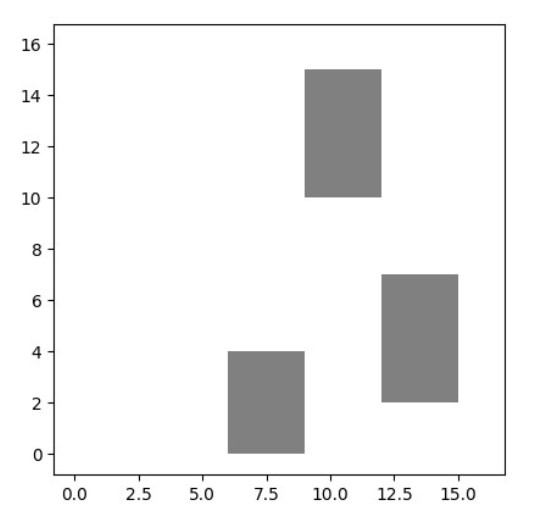
\includegraphics[width=.7\textwidth]{map_init.jpg}
    \caption{Initialisierte Karte mit Hindernissen\\}   
    \label{fig:map_init}
\end{figure}

Die Menge, in der sich der Roboter bewegen darf, ergibt sich aus der Gesamtzahl der Karte \emph{K} und den Hindernissen innerhalb der Karte \emph{H}:
\[K\_frei = K - H\]

Als Nächstes wird, wie bereits in \autoref{ch:algo} beschrieben, die Population initialisiert. Für unseren Fall wird der Bienen Algorithmus nicht verwendet, um einen optimalen Punkt zu finden, sondern um den optimalen Pfad zu finden. Dabei bildet jede Biene einen Pfad ab. Die Pfade bestehen aus \emph{k} vielen Punkten in Form eines Tupels \emph{(x,y)}. Jeder Pfad wird mit den Koordinaten \emph{(0,0)} initialisiert und muss am Ende am Ziel \emph{(16,16)} ankommen. Die Funktion iteriert von \emph{i = 1} bis \emph{k}, da der erste Punkt des Pfades bereits gesetzt ist:

\begin{minted}{python}
def init_population():
    k=7
    i = 1
    path = [(0,0)]
    goal = (16,16)
 while i <= k:
    x = int(random.uniform(0, map_width))
    y = int(random.uniform(0, map_height))
    position = (x,y)
    if is_feasible(position, path[i-1],obstacle_list=obstacle_list):
        path.append((x,y))
        i+=1
    else: 
        x = int(random.uniform(0, map_width))
        y = int(random.uniform(0, map_height))
        position = (x,y)
            
 # Wirf Pfad weg falls das Ziel nach 10 Schritten nicht erreicht ist.
 count = 0
 while not is_feasible(goal,path[i-1],obstacle_list=obstacle_list):
    count += 1
    x = int(random.uniform(0, map_width))
    y = int(random.uniform(0, map_height))
    if is_feasible((x,y), path[i-2], obstacle_list=obstacle_list):
        path[i-1] = (x,y)
    if count > 10:
        return initPopulation()   
    
 path.append(goal)
 return  path
\end{minted}
\vspace*{-3mm}
\captionof{listing}{init\_population Funktion \label{fig:init}}
\vspace*{3mm}

Im Code, der in der Code Darstellung \ref{fig:init} gezeigt wird, wird die stetige Gleichverteilung, auch uniform distribution function genannt, verwendet. Die Gleichverteilungsfunktion ist eine Wahrscheinlichkeitsverteilungsfunktion, die angibt, wie wahrscheinlich es ist, dass eine Zufallsvariable einen bestimmten Wert innerhalb eines bestimmten Intervalls annimmt.
Die Gleichverteilungsfunktion ordnet jedem Wert innerhalb des Intervalls die gleiche Wahrscheinlichkeit zu. Das bedeutet, dass jede Zahl innerhalb des Intervalls mit gleicher Wahrscheinlichkeit gezogen wird.\\
Die Formel für die stetige Gleichverteilung lautet:
\[f(x) = 1/(b-a),\: a \leq x \leq b\]
\[f(x) = 0,\:x < a \:oder\: x > b\]

Dabei ist \emph{a} der untere und \emph{b} der obere Endpunkt des Intervalls \cite{casella2021statistical}. Im Falle dieser Bienen Algorithmus Implementierung wird die stetige Gleichverteilungsfunktion verwendet, um zufällige Pfadpunkte in den Grenzen der Karte zu erstellen.\\
Nach der Erstellung der Punkte muss überprüft werden, ob der Punkt valide ist. Ein Punkt innerhalb eines Pfades \emph{P} wird als valide angesehen, wenn die folgenden Bedingungen erfüllt sind \cite{Darwish2018}:

\[1. \quad P \cap H = \emptyset \quad\]
\[2. \quad \forall i, \forall j \quad \overline{p_i p_j} \cap H = \emptyset\]

Aus diesen zwei Formeln kann man ableiten, dass in einem validem Pfad weder ein Punkt innerhalb eines Hindernisses liegen darf, noch darf eine Verbindung von zwei Punkten der Menge P ein Hindernis aus der Menge \emph{H} schneiden darf.
Die zwei dazugehörigen Funktion sehen wie folgt aus:

\begin{minted}{python}
def pointInsideObstacle(point, obstacle):
    # Überprüfen, ob der Punkt innerhalb des Hindernisses liegt
    for obs in obstacle:
        if point[0] == obs[0] and point[1] == obs[1]:
            return True
                
    return False
\end{minted}
\vspace*{-3mm}
\captionof{listing}{Überprüfen, ob der Punkt in einem Hindernis liegt}
\vspace*{3mm}

\begin{minted}{python}
def intersects(point1, point2, obstacle):
    # Überprüfen, ob die Strecke von point1 zu point2 das Hindernis schneidet

    x_min = min(point1[0], point2[0])
    x_max = max(point1[0], point2[0])
    y_min = min(point1[1], point2[1])
    y_max = max(point1[1], point2[1])

    for obs in obstacle:
        if obs[0] >= x_min and obs[0] <= x_max and obs[1] >= y_min and obs[1] <= y_max:
            return True
    return False
\end{minted}
\vspace*{-3mm}
\captionof{listing}{Überprüfen, ob Schnittpunkt existiert}
\vspace*{3mm}

Aus diesen zwei Funktionen setzt sich die Funktion \emph{is\_feasible()} zusammen, die in der Methode \emph{init\_population()} verwendet wird. Ein neuer Punkt wird also nur hinzugefügt, falls \emph{is\_feasible} wahr ist. Eine Ausnahme die existiert entsteht bei dem Anfügen des letzten Punktes \emph{(16,16)}. Es ist möglich, dass der letzte generierte Punkt des Pfades keine valide Verbindung zu dem Zielpunkt herstellen kann, da immer ein Hindernis im Weg ist. In diesem Falle wird der letzte Punkt des Pfades wieder ersetzt durch einen neuen Punkt. Im Anschluss wird überprüft, ob dieser Punkt auf gültigen Weg zum Ziel kommt. Falls dies nach 10 Versuchen nicht funktioniert, wird der Pfad verworfen und neu initialisiert. Diese Variante stellte sich nach vermehrten Überprüfungen als die effizienteste Möglichkeit heraus.\\

Für die weiteren Schritte des Bienen-Algorithmus wird eine Bewertungsfunktion benötigt. Die Bewertung eines Pfades wird mithilfe des Euklidischen Abstands berechnet:
\[f = \sum_{i=1}^{n-1} \sqrt{(x_{i+1} - x_i)^2 + (y_{i+1} - y_i)^2}\]

Der Euklidische Abstand berechnet den Abstand zwischen zwei Punkten innerhalb einer Ebene \cite{Friedrich2019}. Dies wird für jeden Punkt durchgeführt und aufsummiert. Die passende Funktion dazu sieht wie folgt aus:

\begin{minted}{python}
    def evaluate_path(path):
        x_points = []
        y_points= []
        for i in range(len(path)):
            x, y = path[i]
            x_points.append(x)
            y_points.append(y)
        i=1
        total_distance= 0
        while i < len(path)-1:
            total_distance += np.sqrt((x_points[i+1] - x_points[i]) **2 + (y_points[i+1] - y_points[i])**2)
            i+=1
            return total_distance
\end{minted}
\vspace*{-3mm}
\captionof{listing}{Evaluierungsfunktion}
\vspace*{3mm}

In Kombination mit der Evaluierungsfunktion wird die Lokale Suche des Bienen-Algorithmus angewandt, um in einer bestimmten Umgebung, auch Nachbarschaft genannt, zu suchen. Dafür kann die Größe der Nachbarschaft \emph{ngh} beliebig initialisiert werden. Nachfolgend wird für jeden Punkt des Pfades der übergeben wird, außer für Start und Ziel, ein neuer Punkt mithilfe der stetigen Gleichverteilungsfunktion in einer bestimmten Begrenzung erstellt. Dabei muss allerdings sichergestellt werden, dass ein valider Punkt dem Pfad hinzugefügt wird. Falls der Punkt ungültig ist, wird ein neuer Punkt erstellt. Zum Schluss der Funktion wird überprüft, ob die Fitness des neuen Pfades höher ist als die des alten Pfades. Ist dies der Fall, wird der Pfad aktualisiert. Auf diese Weise wird versucht, die bestehenden Pfade zu optimieren.   

\begin{minted}{python}
    def local_search(solution, fitness):
        ngh = 2
        i = 1
        while i <= len(solution) - 2:
         count= 0
         new_solution = solution.copy()
         new_point =  (int(random.uniform(solution[i][0]-ngh, solution[i][0]+ngh)),int(random.uniform(solution[i][1]-ngh, solution[i][1]+ngh)))
         new_solution[i] = new_point
         while not path_is_feasible(new_solution):
            new_point =  (int(random.uniform(solution[i][0]-ngh, solution[i][0]+ngh)),int(random.uniform(solution[i][1]-ngh, solution[i][1]+ngh)))
             new_solution[i] = new_point 
             count +=1
             if count > 20:
                return solution
            new_fitness = evaluate_path(new_solution)
            if new_fitness < fitness:
                solution = new_solution
            i+= 1
        return solution
\end{minted}
\vspace*{-3mm}
\captionof{listing}{Lokale Suche des Bienen-Algorithmus}
\vspace*{3mm}

Neben der lokalen Suche findet eine globale Suche statt. Hier werden erneut randomisiert eine Menge an Pfaden erstellt und per Evaluationsfunktion bewertet. Dieses Mal wird allerdings nicht die stetige Gleichverteilungsfunktion verwendet. Stattdessen wird eine zufällige Stelle im Pfad ausgewählt und eine zufällige Änderung generiert. Diese neu-erstellten Pfade werden im Anschluss zurückgegeben und zur Gesamtmenge der gefunden Pfade hinzugefügt.

\begin{minted}{python}
    def generate_new_solutions(solutions, best_solution):
        new_solutions = []
        for solution in solutions:
            # Wenn die Lösung mit der besten Lösung übereinstimmt, wird sie übersprungen
            if solution == best_solution:
                continue
            
            # Zufällige Stelle im Pfad auswählen
            index = random.randint(1, len(solution)-2)
            
            # Neue Lösung generieren durch zufällige Änderung an der ausgewählten Stelle
            new_solution = solution.copy()
            new_x = new_solution[index][0] 
            new_y = new_solution[index][1] 
            new_solution[index] = (new_x, new_y)
            
            # Neue Lösung zur Lösungsmenge hinzufügen
            new_solutions.append(new_solution)
        
        return new_solutions
\end{minted}
\vspace*{-3mm}
\captionof{listing}{Globale Suche des Bienen-Algorithmus}
\vspace*{3mm}

Zuletzt müssen diese Methoden auf die Weise, wie in \autoref{ch:algo} erläutert wurde, in einer Funktion zusammengefügt werden. Diese Funktion nimmt als Parameter die Anzahl an Kundschafter Bienen, die auch als Anzahl der Iterationen gesehen werden kann, und wird wie folgt beschrieben:

\begin{minted}{python}
    def bees_algorithm(num_scouts):
     i=0
     solutions = []
     while i <= num_scouts:    
        path = initPopulation()
        solutions.append(path)
            i+=1
    
     for i in range(num_scouts):
     # Führe Local Search für jede Lösung durch
        for j in range(len(solutions)):
            solutions[j] = local_search(solutions[j], evaluate_path(solutions[j]))
    
        # Berechne Fitness-Werte der Lösungen
        fitnesses = [evaluate_path(solution) for solution in solutions]
    
        # Aktualisiere die beste Lösung (findet niedrigsten Wert im Array)
        best_solution_index = np.argmin(fitnesses)
        best_solution = solutions[best_solution_index]
    
        # Generiere neue Lösungen durch globale Suche
        new_solutions = generate_new_solutions(solutions, best_solution)
    
        # Sortiere Array aufsteigend
        fitnesses = sorted(fitnesses)
    
        # Aktualisiere die Lösungsmenge mit den neuen Lösungen
        solutions[num_scouts:] = new_solutions
    
     return solutions, best_solution
\end{minted}
\vspace*{-3mm}
\captionof{listing}{Gesamtheit des Bienen-Algorithmus}
\vspace*{3mm}

Zu Beginn des Algorithmus wird die Population auf die Anzahl der Kundschafter Bienen initialisiert. Anschließend wird für jeden Pfad die lokale Suche durchgeführt, die Fitness berechnet und die beste Lösung aktualisiert. Zudem wird die globale Suche angewandt und das Array aufsteigend anhand der Fitness-Werte sortiert. Die neu-generierten Fitness-Werte werden nun an den Index der Anzahl von Kundschafter Bienen des Arrays angehängt, damit die Menge der Pfade nicht zu groß wird und somit die Funktion effizienter ist.  
In dieser Implementierung wurde als Stopp-Kriterium die Menge an Iterationen gewählt, jedoch lässt sich dieses beliebig wählen. Ein weiteres sinnvolles Stopp-Kriterium wäre beispielsweise ein bestimmter Fitness-Wert. \\\\
Nach 30 Iterationen hat der Bienen Algorithmus den folgenden Pfad errechnet:
\begin{figure}[H]
    \centering
    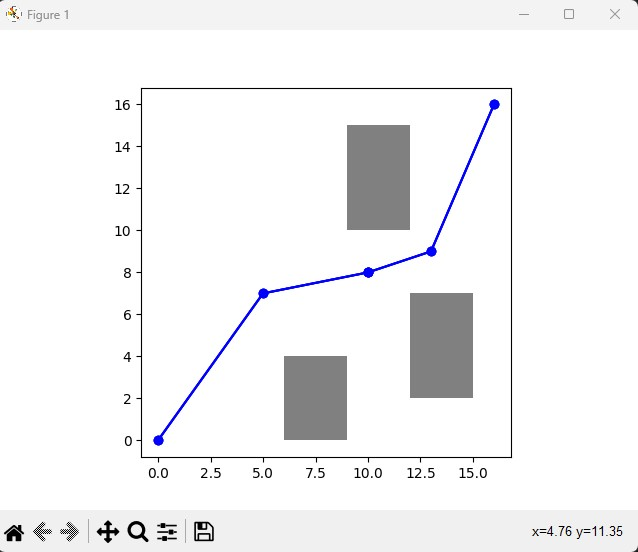
\includegraphics[width=0.7\textwidth]{schnellster_weg.jpg}
    \caption{Schnellster Pfad mit 30 Iterationen\\}   
    \label{fig:schnellster}
\end{figure}

Zur Veranschaulichung, welche Wege der Bienen Algorithmus verwendet hat, wurde die Gesamtheit aller Pfade grafisch dargestellt:
\begin{figure}[H]
    \centering
    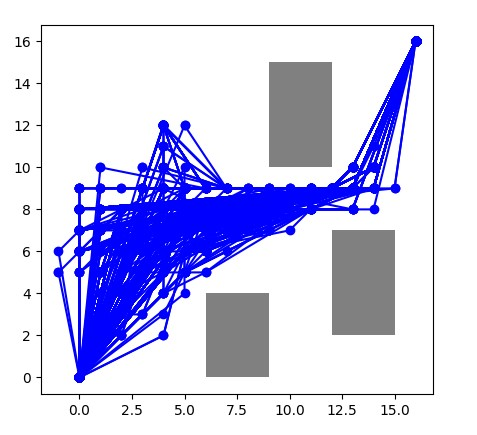
\includegraphics[width=0.7\textwidth]{passende_iterationen.jpg}
    \caption{Initialisierte Karte mit Hindernissen\\}   
    \label{fig:iterationen}
\end{figure}

In \autoref{fig:iterationen} ist die Funktionsweise des Bienen-Algorithmus zu erkennen. Verschiedene Punkte mittels der Lokalen Suche wurden getestet, um den bestmöglichen Weg zu finden.
\chapter{Einplatinencomputer als Roboter}
% LTeX: language=de-DE
\section{Konzepte}
Die theoretischen Grundlagen des Konzepts der Schwarmintelligenz in der Robotik werden in diesem Kapitel erläutert und in Bezug auf eine Anwendung mit Raspberry Pi Einplatinencomputer gebracht. Diese sollen durch einen zufällig generierten Hindernis-Parcours fahren und die vorhandenen Hindernisse hierbei umfahren. Zudem soll durch mehrere Iterationen an Durchläufen die Effizienz der Lösung verbessert werden. Für die Umsetzung und die Lösung des Problems wurden mehrere Ideen und Ansätze entwickelt und in diesem Kapitel erläutert und miteinander verglichen. Außerdem werden die einzelnen Komponenten des Konzepts erläutert und die einzelnen Schritte der Implementierung beschrieben. Die Problemstellung bei allen Konzepten soll sein, dass eine durch X- und Y-Koordinaten definierte Strecke mit einem Hindernis-Parcours so verarbeitet wird, dass durch diese ein Pfad gefunden wird, der Hindernisse vermeidet. Außerdem soll aus diesen gefundenen Pfaden der effizienteste Pfad ermittelt werden.

\subsection{Umsetzung des Konzepts ausschließlich in Code}
Die Umsetzung des Konzepts in Code ist die einfachste und schnellste Möglichkeit, um das Konzept in die Realität umzusetzen. Allerdings ist diese Variante verglichen mit einer Umsetzung mit Hardware weniger realitätsnah und weist einen geringeren Bezug zum eigentlichen Problem, der mobilen Schwarmintelligenz, auf. Für diesen Ansatz werden keine Hardware-Komponenten benötigt. Das zu lösende Problem soll mithilfe eines künstlichen Schwarmes einen Pfad zu finden, der Hindernisse vermeidet umgesetzt werden. Als Programmiersprache soll Python verwendet werden, da Python durch diverse Module und Bibliotheken, wie zum Beispiel Numpy, Matplotlib oder Scipy, einen Vorteil gegenüber anderen Programmiersprachen bietet, mit denen sich die Umsetzung des Konzepts umständlicher umsetzen ließe. In Code Darstellung \autoref{lst:marix-gen} wird eine Methode für die Erstellung einer 20x20 Matrix exemplarisch dargestellt. Eine solche Matrix kann als eine Art "Karte" verstanden werden, auf der Hindernisse und Wege dargestellt werden können. Die Matrix wird mit Nullen initialisiert und an den Stellen, an denen Hindernisse sein sollen, mit Einsen belegt. Mit den exemplarischen Parametern werden 18 Hindernisse zufällig gesetzt. Die Matrix wird anschließend ausgegeben.

%minted python code
\begin{minted}{python}
import numpy as np

def obstacles():
    """
    Creates a 20x20 grid with obstacles randomly placed.
    Grid containing 1 is an obstacle, containing 0 is empty.
    Returns a numpy array of the grid.
    """
    obs = np.zeros((20,20))
    for i in range(18):
        obs[np.random.randint(20)][np.random.randint(20)] = 1  
  
    return obs
\end{minted}
\vspace*{-3mm}
\captionof{listing}{\label{lst:marix-gen}Matrizen Generierung}
\vspace*{3mm}

Die Abbildung, die mit dem Python Package \textit{matplotlib} erstellt wurde, visualisiert eine Matrix, die durch die in Code Darstellung \autoref{lst:marix-gen} dargestellte Funktion erstellt wurde. Der Startpunkt ist bei den Koordinaten (0/0) als grüner Punkt angezeigt. Das Ziel am Punkt (20/20) als roter Punkt. Die weiße Fläche stellt den freien und somit durchquerbaren Bereich und die schwarzen Flächen den durch Hindernisse blockierten dar. Diese Daten sind die Ausgangslage für einen darauf angewandten Schwarmintelligenz Algorithmus dar, dessen Output den bestmöglichen Pfad durch diese Fläche ermitteln soll, siehe \autoref{fig:Figure_1}.
\begin{figure}[H]
    \centering
    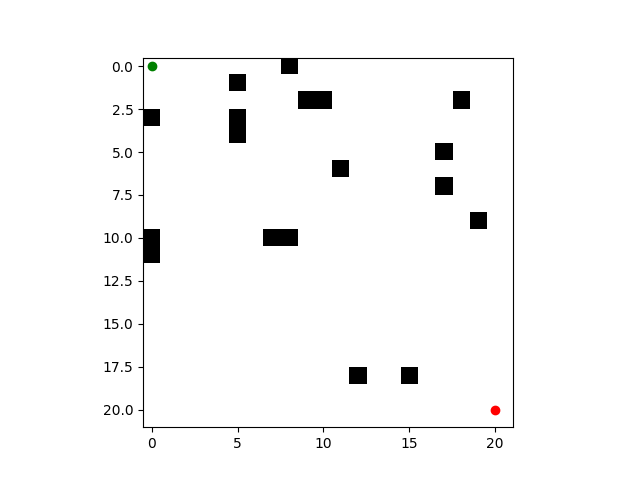
\includegraphics[width=\textwidth]{Figure_1.png}
    \caption{Visualisierung der Matrix}
    \label{fig:Figure_1}
\end{figure}

In Folge der Ermittlung kann der optimale Pfad verwendet werden, um den effizientesten Weg durch die Matrix, beziehungsweise die Hindernisse grafisch darzustellen.

\subsection{Umsetzung des Konzepts in der physischen Variante}
In dieser Implementierung wird ein Schwarmintelligenz-Algorithmus verwendet, um einen optimalen Pfad basierend auf Daten aus der realen Umgebung zu finden. Im Gegensatz zur reinen Code-basierten Variante werden die Daten nicht zufällig generiert, sondern von Sensoren des Roboters in der physischen Umgebung erfasst. Denkbar wären hier beispielsweise die Nutzung von Ultraschallsensoren, die an Einplatinencomputer wie dem Raspberry Pi an den vorhandenen GPIO-Pins angeschlossen werden können. Die Sensoren sammeln regelmäßig Daten, die in einer Datenbank gespeichert und periodisch abgefragt werden könnten, um sie dem Schwarmintelligenz-Algorithmus zur Berechnung des optimalen Pfades zur Verfügung zu stellen. Der Algorithmus liefert dann den optimalen Pfad, den der Roboter durch die Umgebung nutzen kann. Dieser soll dann in der Lage sein, den Pfad so zu durchfahren, dass er nicht mehr auf die Sensoren zur Erkennung der Hindernisse angewiesen ist. Sowohl beim Erlangen der Daten, wobei der Roboter an einem Startpunkt beginnt, die Umgebung zu durchfahren, als auch beim Durchfahren ohne die Sensoren, müssen die Koordinaten des Roboters zum jeweils aktuellen Zeitpunkt bestimmt werden können. Dies ist nur dann möglich, wenn anhand der Umdrehungen der Servomotoren, die zur Fortbewegung genutzt werden, ermittelt werden kann, wie weit und in welche Richtung sich ein Roboter jeweils fortbewegt hat. Für die Ermittlung wird hierfür weiterhin die Größe der verwendeten Räder benötigt. Sind diese beiden Messgrößen bekannt, können anhand dieser die Position und auch Anweisungen zum Fahren übermittelt werden.
\begin{figure}
    \centering
    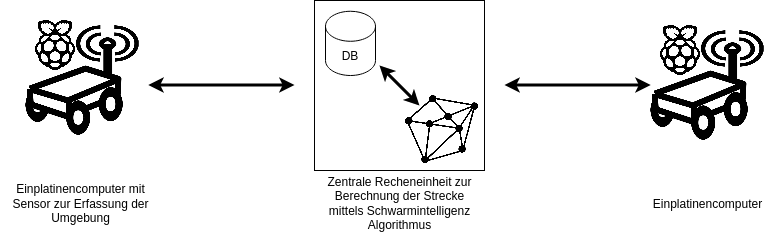
\includegraphics[width=\textwidth]{draw_io_overview_robot.png}
    \caption{Übersicht physische Variante}
    \label{fig:Figure_2}
\end{figure}

Die Qualität der Daten hängt hierbei stark von der verwendeten Hardware ab. Zum einen, weil anhand von Umdrehungen der Servomotoren bestimmt wird, wo sich ein Roboter zum jeweiligen Zeitpunkt befindet und zum anderen von der Genauigkeit der verwendeten Ultraschallsensoren, wenn diese Hindernisse in ihrer Umgebung detektieren. Als zusätzlicher Schritt, welcher bei der Code-basierten Variante nicht anfällt, ist es in dieser Umsetzung notwendig, die erfassten Daten in eine Form zu bringen, die der Schwarmintelligenz-Algorithmus verarbeiten kann. Denkbar wäre hier ebenfalls die Nutzung von Bibliotheken wie beispielsweise `numpy`, um eine Matrix in der Größe des Kartenbereichs zu erstellen. Anhand der aktuellen Position des erfassenden Raspberry Pi Roboters könnten in Abhängigkeit des Abstands zu einem Hindernis die entsprechenden X- und Y-Koordinaten in der Matrix auf 1 gesetzt werden. Eine solche Matrix könnten dann wie in der Code-basierten Variante an den Schwarmintelligenz-Algorithmus zur Verarbeitung übergeben werden.

\subsection{Umsetzung des Konzepts hybrider Variante}
Bei der Umsetzung in hybrider Variante handelt es sich um ein gemischtes Vorgehen aus der reinen Code-basierten Variante und der physischen Variante. Die Daten der zu verarbeitenden Umgebung werden wie bei der Code-basierten Variante durch einen Algorithmus generiert. Nach Verarbeitung der Daten erfolgt jedoch ein Schritt in die physische Umsetzung. Der durch den verwendeten Schwarmintelligenz Algorithmus ermittelte Pfad wird nach der Verarbeitung in Instruktionen übersetzt, die der Roboter in der physischen Umgebung ausführen kann. Hierfür ist eine Verbindung zwischen dem Algorithmus und dem Roboter notwendig. Diese kann beispielsweise durch eine WLAN-Verbindung hergestellt werden. Weiterhin muss eine Schnittstelle geschaffen werden, über welche der Client, der den Algorithmus und die Berechnungen ausführt, mit dem Roboter kommunizieren kann. Wenn auf das Kriterium der Echtzeit verzichtet werden kann, eignet sich hierfür eine reguläre API Schnittstelle. Der Raspberry würde in diesem Fall einen Endpunkt darstellen, an den Instruktionen in Form des gewählten Datenformats wie beispielsweise JSON oder XML gesendet werden. Diese Schnittstelle würde sich zudem auch für die Übermittlung von Signalen wie Start, Stopp oder Reset eignen.
\begin{figure}[H]
    \centering
    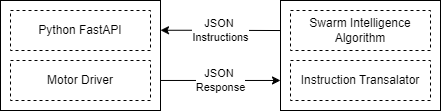
\includegraphics[width=\textwidth]{hybrid-diagram.png}
    \caption{Übersicht hybride Variante}
    \label{fig:overview-hybrid}
\end{figure}

\section{Auswahlkriterien für das verwendete Vorgehen}
Bei der Auswahl von Kriterien für den Vergleich zwischen der reinen Code-basierten Implementierung, der physischen Implementierung und der hybriden Implementierung des Konzepts der mobilen Schwarmintelligenz werden die folgenden Aspekte berücksichtigt:
\begin{itemize}
    \item Realitätsnähe: Realitätsnähe im Kontext der Implementierung eines Schwarmverhaltens bezieht sich auf die Fähigkeit der Implementierung, das tatsächliche Verhalten des Schwarmes in der realen Umgebung genau vorherzusagen. Es geht darum, wie nahe die Simulation der realen Umgebung kommt und wie gut die Implementierung die Gegebenheiten und Bedingungen der realen Welt berücksichtigt.
    \item Komplexität: Komplexität im Kontext der Implementierung sowie einer möglichen physischen Umsetzung bezieht sich auf den Schwierigkeitsgrad der Implementierung des Schwarmintelligenz-Algorithmus sowie der physischen Umsetzung. Hierbei werden die Kriterien Programmieraufwand, zusätzlich benötigte Kenntnisse und die Komplexität der benötigten Hardware berücksichtigt.
    \item Kosten: die Kategorie Kosten bezieht sich in erster Linie auf eine Implementierung der physischen Variante. Hierbei werden die Kosten für die benötigte Hardware berücksichtigt. Es soll erwähnt werden, dass eine Implementierung mit bereits vorhandenen und durch die Lehrstätte zur Verfügung gestellten Ressourcen durchgeführt werden soll.
    \item Skalierbarkeit: Skalierbarkeit bezieht sich auf die Fähigkeit der Implementierung, auf größere oder kleinere Umgebungen angepasst zu werden. Das bedeutet, dass die Implementierung in der Lage sein sollte, auf unterschiedliche Schwarmgrößen, räumliche Gegebenheiten, unterschiedliche Sensordaten oder andere Anforderungen anpassbar zu sein.
    \item Geschwindigkeit: Geschwindigkeit bezieht sich in diesem Zusammenhang auf die Fähigkeit des Algorithmus, Eingabedaten schnell zu verarbeiten und Entscheidungen zu treffen. Eine Implementierung mit hoher Geschwindigkeit kann schnell auf Änderungen in der Umgebung oder auf neue Anforderungen reagieren und somit effektiver arbeiten.
    \item Visualisierung: Visualisierung bezieht sich darauf, wie die Ergebnisse der Implementierung dargestellt und realitätsnah dargestellt werden können. Es soll betrachtet werden, wie gut das Verhalten des Schwarmes in der realen Umgebung simuliert werden kann und wie gut die Ergebnisse der Implementierung dargestellt werden können.
\end{itemize}

\begin{table}[H]
    \renewcommand{\arraystretch}{1.2}
    \caption{Entscheidungsmatrix: verwendetes Konzept}
    \label{tab:decision-matrix}
    \begin{tabularx}{\textwidth}{|X|X|X|X|}
        \hline
        & \textbf{Code-basiert} & \textbf{Physisch} & \textbf{Hybrid} \\
        \hline
        \textbf{Kriterium} & Punkte & Punkte & Punkte \\
        \hline
        Realitätsnähe & 1 & 5 & 3 \\
        \hline
        Komplexität & 4 & 1 & 3 \\
        \hline
        Kosten & 5 & 3 & 4 \\
        \hline
        Skalierbarkeit & 4 & 2 & 3 \\
        \hline
        Geschwindigkeit & 4 & 2 & 3 \\
        \hline
        Visualisierbarkeit & 2 & 5 & 4 \\
        \hline
        \rowcolor{gray!50}
        \textbf{Summe} & 20 & 18 & 20 \\
        \hline
    \end{tabularx}
\end{table}

Die Punkte der einzelnen Kriterien wurden in einer Skala von 1 bis 5 vergeben. Dabei steht 1 für die schlechteste Bewertung und 5 für die beste Bewertung. Die Summe der Punkte der einzelnen Kriterien ergibt die Gesamtpunktzahl für das jeweilige Konzept. Die ermittelten Punkte liegen wie in \autoref{tab:decision-matrix} alle sehr nah beieinander. Während die Umsetzung des Vorhabens in der physischen Variante einen erhöhten Aufwand und gegenüber den anderen Vorgehensweisen mit einer deutlich höheren Komplexität einhergeht, bietet sie gleichzeitig die beste Realitätsnähe. Die Umsetzung in der Code-basierten Variante ist hingegen mit einem geringeren Aufwand verbunden, bietet jedoch die geringste Realitätsnähe. Die Umsetzung in der hybriden Variante bietet eine gute Realitätsnähe und ist mit einem vergleichbaren Aufwand verbunden. Eine Umsetzung in der hybriden Variante wird daher als Basis für die weitere Implementierung des Vorhabens verwendet. 

\section{Hardware}
In diesem Abschnitt werden die verwendeten Hardware-Komponenten für die Umsetzung der hybriden Variante beschrieben. Es ist zu erwähnen, dass bei der gewählten und verwendeten Hardware vorzugsweise auf Materialien zurückgegriffen wurde, die bereits durch die Lehrstätte zur Verfügung gestellt wurden. Möglicherweise gibt es bessere Alternativen, die zum Zeitpunkt der Umsetzung jedoch nicht zur Verfügung standen. Die verwendeten Hauptkomponenten sind ein Raspberry Pi 3, ein Grove Base HAT, ein Servo Motor und ein eigens dafür konstruiertes und anschließend mit einem 3D-Drucker angefertigtes Gehäuse, das alle Komponente vereint. Die Komponenten sind in \autoref{fig:hardware} dargestellt.

\begin{figure}[ht]
    \centering
    \begin{subfigure}[b]{0.45\textwidth}
      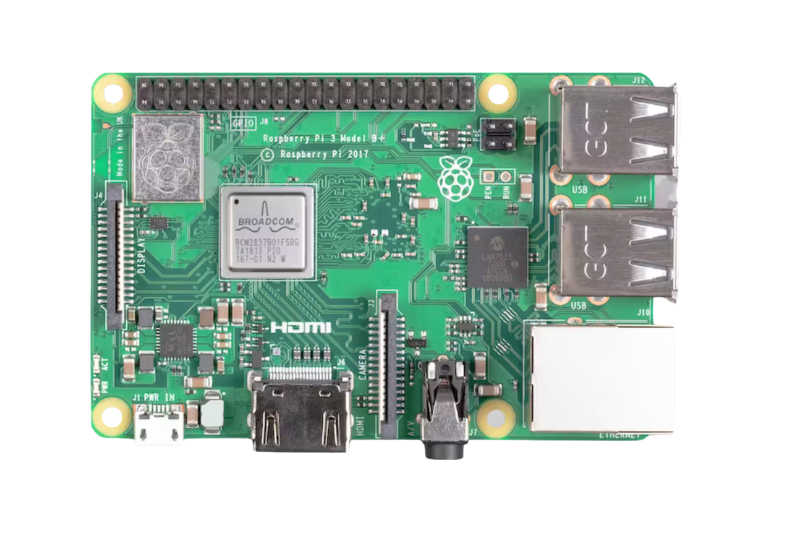
\includegraphics[width=\textwidth]{raspi.png}
      \caption{Raspberry Pi 3 \cite{raspberry-pi}}
    \end{subfigure}
    \hspace{1cm}
    \begin{subfigure}[b]{0.45\textwidth}
      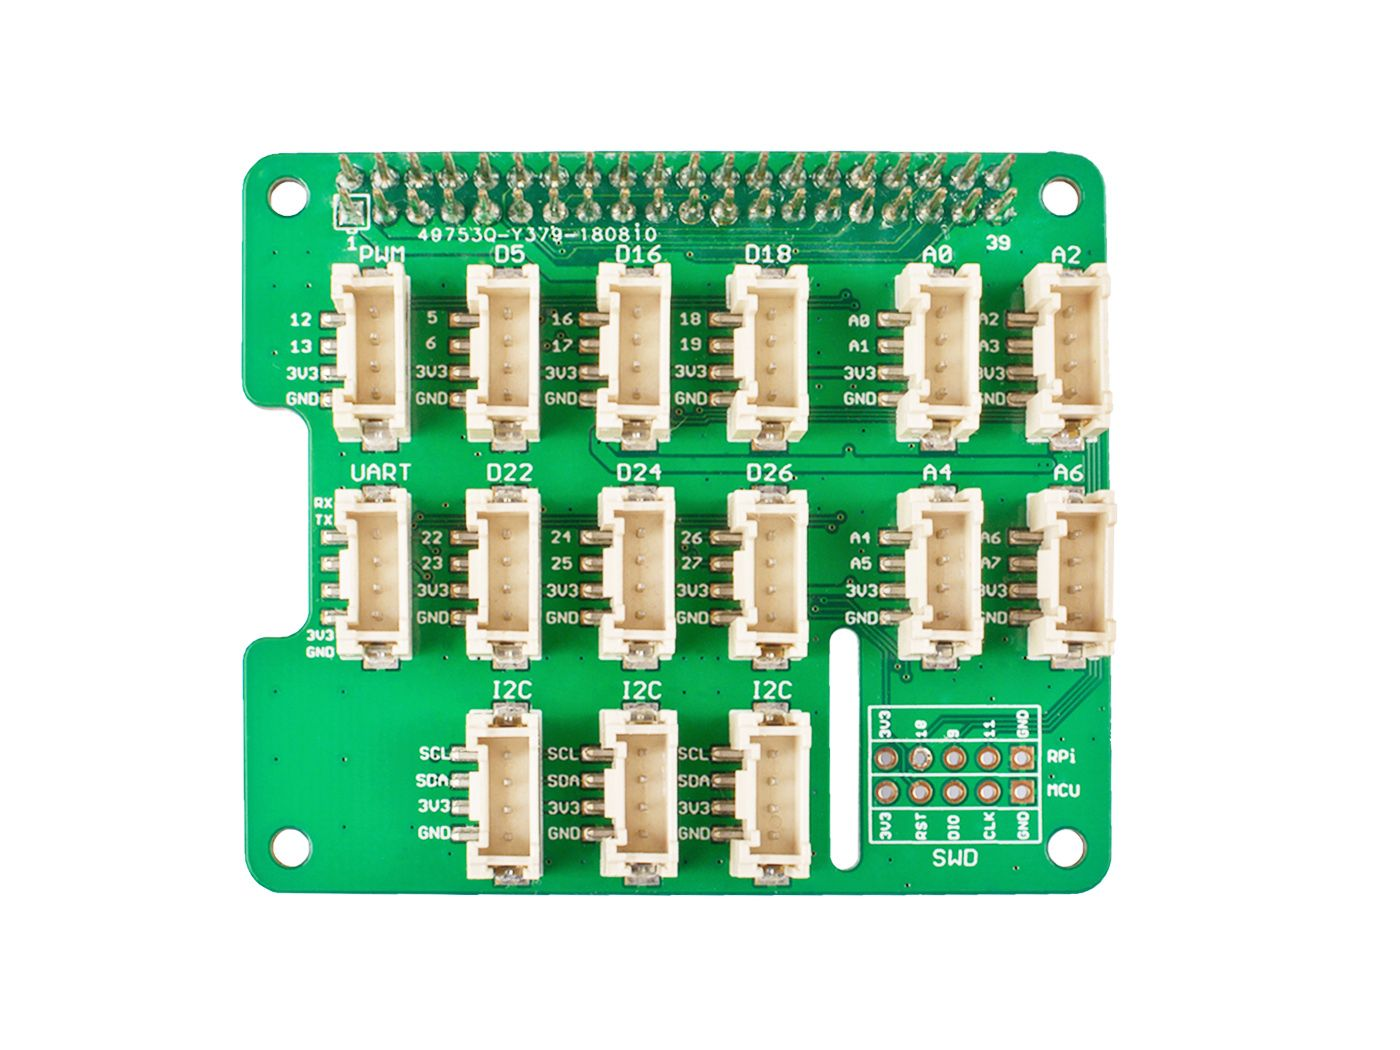
\includegraphics[width=\textwidth]{base-hat.jpg}
      \caption{Grove Base HAT \cite{seeedstudio} \label{fig:base-hat}}
    \end{subfigure}
    \vskip\baselineskip
    \begin{subfigure}[b]{0.45\textwidth}
        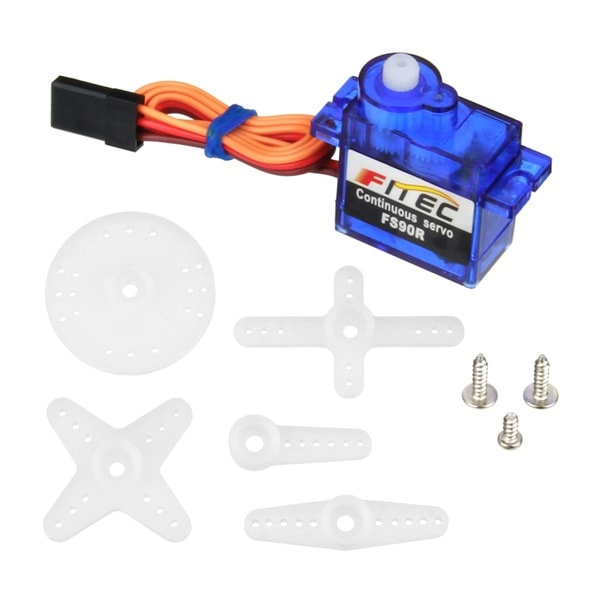
\includegraphics[width=\textwidth]{servo.jpg}
        \caption{Servomotor \cite{addicore_fs90r_micro_servo} \label{fig:servo}}
      \end{subfigure}
      \hspace{1cm}
      \begin{subfigure}[b]{0.45\textwidth}
        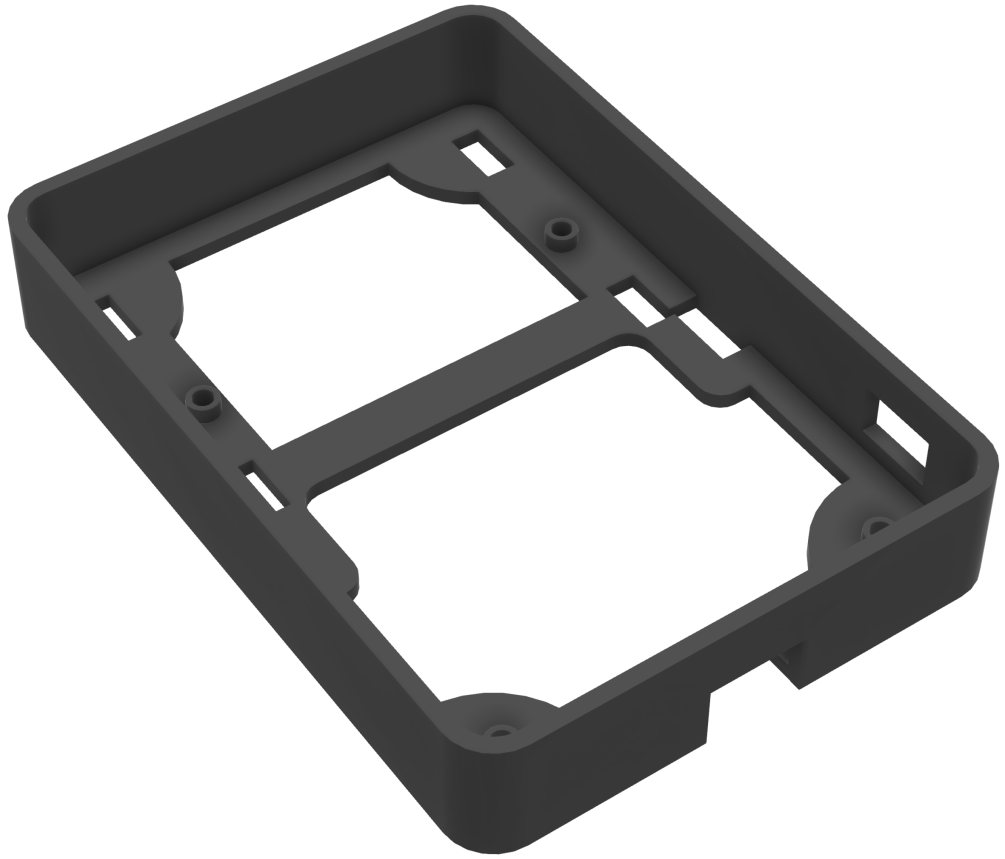
\includegraphics[width=\textwidth]{case.png}
        \caption{Roboter Gehäuse \label{fig:case}}
      \end{subfigure}
    \caption{Verwendete Bauteile \label{fig:hardware}}
\end{figure}

Der Raspberry Pi dient hierbei als Einplatinencomputer, der die Steuerung des Roboters übernimmt. Der Grove Base HAT, in \autoref{fig:base-hat} dargestellt, bietet die Möglichkeit verschiedene Sensoren und Aktoren anzuschließen. Servomotoren, wie in \autoref{fig:servo} dargestellt, dienen hierbei als Antrieb des Roboters. Das Gehäuse, in \autoref{fig:case} dargestellt, vereint alle Komponenten und bietet eine einfache Montage und Demontage der einzelnen Komponenten. Die Wahl des Servomotors ist aufgrund der geringen Größe und der niedrigen benötigten Versorgungsspannung auf ein Modell dieser Bauart gefallen. Außerdem sind diese Art von Servomotoren günstig erhältlich sowie energieeffizient \cite{Sustek2017}. Die Wahl des Grove Base HAT ist aufgrund der einfachen Verwendung und der Möglichkeit, verschiedene Sensoren und Aktoren anzuschließen, auf dieses Modell gefallen. Bei diesem Bauteil handelt es sich um eine Addon Board, das es erlaubt, Bauteile wie Sensoren und Aktoren über einen einfachen Steckverbinder anzuschließen \cite{seeedstudio}.


\section{Steuerung und Kommunikation}
Für die Kommunikation des Roboters stehen verschiedene Übertragungs- und Kommunikationsmöglichkeiten zur Verfügung. Aufgrund der Anforderung, dass das Gerät mobil betrieben werden soll, eignet sich eine kabellose Variante.

Vergleichen werden hierfür die Möglichkeiten MQTT, REST API und Web Socket. Für den Anwendungsfall relevant sind die folgenden Eigenschaften:
\begin{itemize}
  \item Einfache Implementierung
  \item Keine zusätzliche Hardware notwendig
  \item Flexibilität
  \item Skalierbarkeit
  \item Zuverlässigkeit
\end{itemize}

Während sich Kriterien für den Einsatz von Robotik hauptsächlich auf eine hohe Zuverlässigkeit, geringe Latenzen sowie eine hohe Flexibilität beziehen \cite{AMARAN2015400}, werden im Rahmen dieser studentischen Arbeit andere Kriterien als relevant angesehen, mit unter, weil diese für die Umsetzung des Vorhabens eine Erleichterung mit sich bringen. So ist die einfache Implementierung ein wichtiges Kriterium, da die Umsetzung in einer begrenzten Zeit erfolgen soll. Die zu verwendende Hardware soll sich, wenn möglich, auf bereits vorhandene Komponenten beschränken. Flexibilität ist insofern relevant, als bei der Umsetzung des Vorhabens eine hohe Anpassungsfähigkeit an die Umgebung gewünscht ist. Wenn Änderungen notwendig werden, soll diese möglichst einfach umsetzbar sein, ohne dass die gesamte Umsetzung neu durchgeführt werden muss. Skalierbarkeit soll möglich sein, sodass das System bei einer Erweiterung der Anzahl an Geräten, auf das es verteilt wird, in gleicher Weise funktionieren soll. Zuverlässigkeit ist ein wichtiges Kriterium, da die Kommunikation zwischen den einzelnen Geräten nicht unterbrochen werden darf.
\begin{table}[H]
  \renewcommand{\arraystretch}{1.2}
  \caption{Entscheidungsmatrix: Verwendete Kommunikationsprotokolle}
  \label{tab:decision-matrix-communication}
  \begin{tabularx}{\textwidth}{|X|X|X|X|}
      \hline
      & \textbf{MQTT} & \textbf{REST API} & \textbf{Web Socket} \\
      \hline
      \textbf{Kriterium} & Punkte & Punkte & Punkte \\
      \hline
      Einfache Implementierung & 2 & 4 & 3 \\
      \hline
      Keine zusätzliche Hardware & 1 & 5 & 5 \\
      \hline
      Flexibilität & 5 & 3 & 4 \\
      \hline
      Skalierbarkeit & 4 & 4 & 4 \\
      \hline
      Zuverlässigkeit & 5 & 4 & 4 \\
      \hline
      \rowcolor{gray!50}
      \textbf{Summe} & 17 & 20 & 20 \\
      \hline
  \end{tabularx}
\end{table}

Die Punkte der einzelnen Kriterien wurden in einer Skala von 1 bis 5
vergeben. Dabei steht 1 für die schlechteste Bewertung und 5 für die beste Bewertung. Die Summe der Punkte der einzelnen Kriterien ergibt die Gesamtpunktzahl für die jeweilige Technologie.
Obwohl in den Bereichen Robotik und IoT häufig MQTT verwendet wird \cite{AMARAN2015400}, wird es für diese studentische Arbeit nicht in Betracht gezogen. Nicht zuletzt, weil keine Vorkenntnisse der Bearbeitenden vorhanden sind.

\subsection{REST API}
Unter Einbeziehung der in \autoref{tab:decision-matrix-communication} aufgezeigten Ergebnisse der Entscheidungsfindung für eine geeignete Möglichkeit der Kommunikation mit dem verwendeten Raspberry Pi Einplatinencomputer, fällt die Wahl für die Implementierung einer REST API Schnittstelle auf die in Python zu implementierende Lösung \textit{FastAPI} \cite{tiangolo_fastapi_features}. In \autoref{fig:apidocs} werden die für das Vorhaben benötigten API-Endpunkte in Form einer durch die Umsetzung automatisch generierten API-Dokumentation aufgezeigt.
\begin{figure}[H]
  \centering
  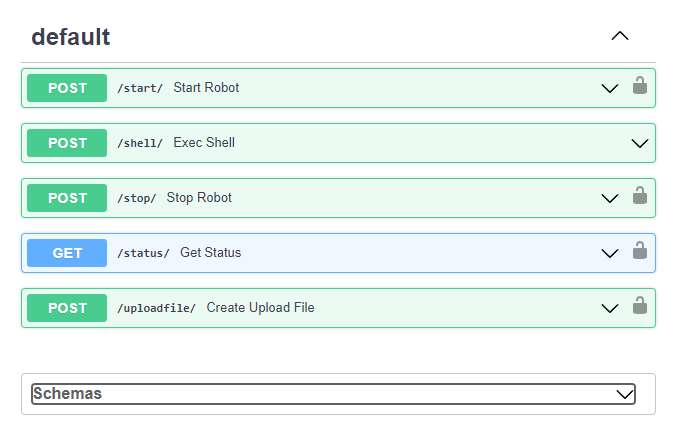
\includegraphics[width=\textwidth]{api-docs.png}
  \caption{API Docs}
  \label{fig:apidocs}
\end{figure}

Bei den implementierten Endpunkten handelt es sich um die in \autoref{fig:apidocs} dargestellten. Folgende Funktionalitäten werden durch die Endpunkte bereitgestellt:

\begin{itemize}
  \item \textbf{/start/}: dieser Endpunkt stellt die Funktionalität bereit, den Roboter unter Verwendung einer vorhandenen Instruktions-Datei zu starten. Dieser Vorgang wird nur dann ausgeführt, wenn noch kein aktiver Fahrvorgang existiert. Ist keine valide Instruktions-Datei vorhanden wird der Vorgang ebenfalls nicht gestartet.
  \item \textbf{/stop/}: dieser Endpunkt stellt die Funktionalität bereit, einen fahrenden Roboter zu stoppen und somit die Ausführung einer Instruktions-Datei zu unterbrechen. Diese Funktion könnte dann von Relevanz sein, wenn das Fahrverhalten Fehler aufweist.
  \item \textbf{/shell/}: dieser Endpunkt liefert die Möglichkeit, reguläre Linux Shell Befehle über die API-Schnittstelle an den verwendeten Raspberry Pi zu übermitteln. Dies ist sowohl mit einzelnen, als auch Aneinanderreihung von Befehlen und Parametern möglich. Hiermit kann der Raspberry beispielsweise neu gestartet oder heruntergefahren werden. Einen Vorteil bietet der Endpunkt insofern, als keine gesonderte SSH-Verbindung für das Ausführen kleinerer Befehle aufgebaut werden muss.
  \item \textbf{/status/}: dieser Endpunkt stellt eine Funktionalität bereit, mit der der aktuelle Status eines Roboters angefragt werden kann. Zum Zeitpunkt der Implementierung beschränkt sich dieser lediglich auf die beiden Zustände \textit{active} und \textit{inactive}. Weiterhin denkbar wären jedoch die Bereitstellung zusätzlicher Informationen wie dem Fortschritt einer aktuell abzuarbeitenden Instruktions-Datei.
  \item \textbf{/uploadfile/}: dieser Endpunkt stellt die Funktionalität bereit, mit der ein Anwender die Instruktionen, der durch den Schwarmintelligenz-Algorithmus errechneten Pfadinformationen, übertragen kann. Es ist zu beachten, dass ein Roboter jeweils einen Datensatz an Instruktionen verarbeiten kann und zum aktuellen Zeitpunkt keine Warteschlange für die Aneinanderreihung mehrerer Instruktions-Dateien vorgesehen ist. Wählt der Anwender eine valide Datei für die Übertragung aus, wird diese nach vorheriger Überprüfung in ein  \textit{/tmp/} Verzeichnis übertragen. Möglicherweise bereits existierende Instruktionen werden hierbei überschrieben. Befindet sich der Roboter zum Zeitpunkt der Anfrage im Zustand \textit{active}, ist ein Übermitteln einer neuen Instruktions-Datei nicht möglich. 
\end{itemize}

\subsection{API Sicherheitsaspekte}
Da der durch den Raspberry bereitgestellte Endpunkt eine Möglichkeit bietet, den Raspberry und die daran angeschlossene Hardware zu steuern, gilt es einige Grundsätze zu beachten, dass durch die Implementierung dieser Schnittstelle keine Schwachstellen offengelegt werden. Besonders, da eine Shell-Kommunikation, zur erweiterten Steuerung, sowie dem Sammeln von Debugging-Informationen genutzt werden soll.

\subsubsection*{API Key Authentifizierung}
Eine gängige Maßnahme um API-Endpunkte gegen unberechtigte Nutzung und gegebenenfalls schadhafte Anfragen zu schützen, ist die Implementierung der Abfrage eines API-Keys zur Authentifizierung des Anwenders \cite{De2017}. Aus diesem Grund werden die Routen durch die Authentifizierung mittels eines API-Keys geschützt, sodass eine Ausführung nur dann erlaubt ist, wenn ein valider API Key im Header der jeweiligen Anfrage mitgeliefert wird. Eine valide Anfrage, wie sie vom Endpunkt des Raspberry Pis akzeptiert wird, ist in \autoref{lst:curl} dargestellt. Die verwendete Länge des API Keys wird anhand der Empfehlungen aus \cite{NISTSP800-57pt3r1} gewählt und in der Implementierung umgesetzt. Weiterhin wird der API Key nicht in den geschriebenen Code, sondern in die Systemumgebungsvariablen des ausführenden Systems integriert. Innerhalb des Codes wird diese Variable zu dem Zeitpunkt aufgerufen, wenn eine Überprüfung des API Keys notwendig ist.

\inputminted{text}{{assets/code/curl.sh}}
\vspace*{-3mm}
\captionof{listing}{\label{lst:curl}Curl API Request}
\vspace*{3mm}

Eine Methode eines API-Endpunkts, der durch die Abfrage des API Keys abgesichert ist, ist in \autoref{lst:sec-api} dargestellt.

\inputminted{python}{{assets/code/run-shell.py}}
\vspace*{-3mm}
\captionof{listing}{\label{lst:sec-api}Geschützter Endpunkt}
\vspace*{3mm}

\subsubsection*{Validierung der JSON Instruktionen}
Neben API-Anfragen, die eine direkte Auswirkungen auf angeschlossene Hardware-Elemente haben können, handelt es sich bei dem Endpunkt \textit{uploadfile} um eine Schnittstelle, bei dem der Anwender einen Request ausführen kann, bei dem der Anwender eine JSON-Datei auf den Raspberry Pi übertragen kann. Die Möglichkeit dieses Vorgangs bietet potenziell die Möglichkeit, Dateien und Dateiformate zu übertragen, welche nicht dafür vorgesehen sind oder sogar schadhafte Auswirkungen auf das Zielsystem haben können. Aus diesem Grund wird eine Validierung der JSON-Datei als notwendig betrachtet. Zudem bietet sich hierdurch der Vorteil, dass die Struktur und der Aufbau der JSON-Datei im gleichen Zug überprüft werden kann und so von vornherein keine inkorrekten Dateien, bei deren Ausführung es zu Fehlern kommen könnte, auf den Raspberry Pi übertragen werden können.

\inputminted{python}{{assets/code/json-check.py}}
\vspace*{-3mm}
\captionof{listing}{\label{lst:json-check}API JSON Validierung}
\vspace*{3mm}

\section{Verarbeitung der Instruktionen}
Damit der Roboter übermittelte Instruktionen umsetzen kann und sich der Roboter fortbewegen kann, wird eine Möglichkeit benötigt, um mit den verwendeten Motoren zu kommunizieren. Hierfür wird durch die Lehrstätte eine Hardware-Komponente bereitgestellt, die diese Anbindung vereinfacht. Das dafür verwendete Grove Base Hat, in \autoref{fig:base-hat} dargestellt, bietet die Möglichkeit mittels einem einzigen Stecker die Anschlüsse \textit{GND, VCC, Signal} zu verbinden. Bei den Instruktionen, die für den Raspberry Pi Roboter benötigt werden, handelt es sich um die Funktionen vorwärts Fahren, rückwärts Fahren, rechts, sowie links Drehen. Diese Manöver werden folgendermaßen implementiert: Die verwendeten Motoren können sich sowohl vorwärts als auch rückwärts drehen. Für den Vorgang des vorwärts Fahrens werden beide Motoren gleichzeitig in Richtung vorwärts angesteuert. Das gleiche Vorgehen wird für den Vorgang des rückwärts Fahrens mit rückwärts Drehungen umgesetzt. Für die Vorgänge der Rechts- sowie Linksdrehung wird jeweils nur ein Motor zur Zeit angesteuert. Eine Drehung in einem bestimmten Winkel wird implementiert, indem zuvor durch Experimente bestimmt wird, wie viele MS ein Motor angesteuert werden muss, um den Roboter beispielsweise um 90 Grad zu drehen. Die Möglichkeit anderer Winkel wird mit diesem ermittelten Faktor errechnet. Für die vorwärts und rückwärts Bewegung muss durch eine Instruktion eine Zeit in Sekunden angegeben werden, für die der Roboter sich bewegen soll. Nach Ablauf dieser Zeit werden die Motoren gestoppt und es können weitere Instruktionen ausgeführt werden.

\section{Umbau des Einplatinencomputers}
Um alle Komponenten des Roboters miteinander zu vereinen wurde eine Plattform mithilfe der Konstruktionssoftware \textit{Fusion 360} erstellt. Die Anforderungen an dieses Modell sind wie folgt:
\begin{itemize}
  \item Die Plattform muss die Möglichkeit bieten, den Raspberry Pi aufzunehmen und zu fixieren.
  \item Es muss eine Möglichkeit geben, die Motoren zu fixieren.
  \item Die Plattform muss die Möglichkeit bieten, die Anschlusskabel der Motoren und des Raspberry Pi zu verbinden.
  \item Der SD-Kartenslot sowie die USB-Anschlüsse des Raspberry Pi müssen zugänglich sein.
\end{itemize}

\begin{figure}[H]
  \centering
  \begin{subfigure}[b]{0.45\textwidth}
    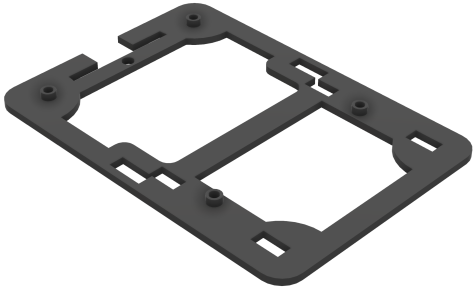
\includegraphics[width=\textwidth]{con-plattform.png}
    \caption{Plattform}
  \end{subfigure}
  \hspace{1cm}
  \begin{subfigure}[b]{0.45\textwidth}
    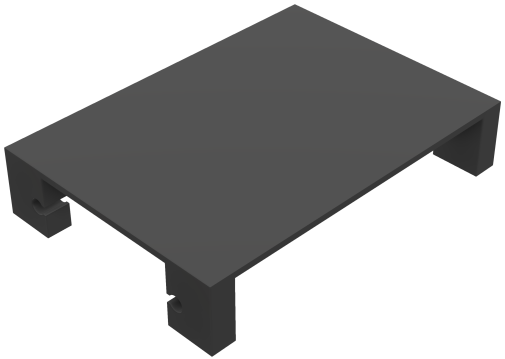
\includegraphics[width=\textwidth]{con-motor-halterung.png}
    \caption{Motor Halterung}
  \end{subfigure}
  \vskip\baselineskip
  \begin{subfigure}[b]{0.45\textwidth}
      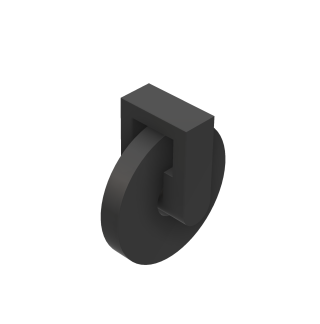
\includegraphics[width=\textwidth]{con-vorderrad.png}
      \caption{Vorderrad}
    \end{subfigure}
    \hspace{1cm}
  \begin{subfigure}[b]{0.45\textwidth}
    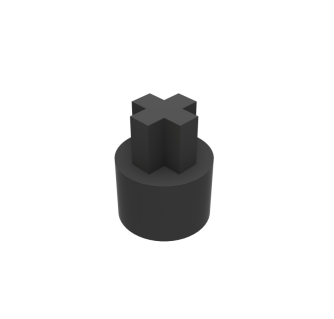
\includegraphics[width=\textwidth]{con-rad-adapter.png}
    \caption{Rad Adapter}
  \end{subfigure}
  \caption{Konstruierte Bauteile \label{fig:konstruktion}}
\end{figure}

Weiterhin müssen an die beiden Motoren die verwendeten Räder angebracht werden. Hierfür wurde ebenfalls ein Adapter konstruiert. Neben den genannten Bauteilen wurde weiterhin ein einzelnes Vorderrad für den Roboter konstruiert. Die Konstruktion der Bauteile ist in \autoref{fig:konstruktion} dargestellt. Nach Fertigstellung sowie mehreren Anpassungen der Konstruktionen wurden die Bauteile mit einem 3D-Drucker hergestellt. Die einzelnen Komponenten wurden miteinander verklebt und anschließend die übrigen Hardware-Komponenten mit Feingewinde-Schrauben befestigt. Der fertige Roboter ist in \autoref{fig:fertiger-roboter} dargestellt. Eine größere Darstellung des Roboters ist zudem dem Anhang in \autoref{sec:darstellungen} zu entnehmen.

\begin{figure}[H]
  \centering
  \begin{subfigure}[b]{0.45\textwidth}
    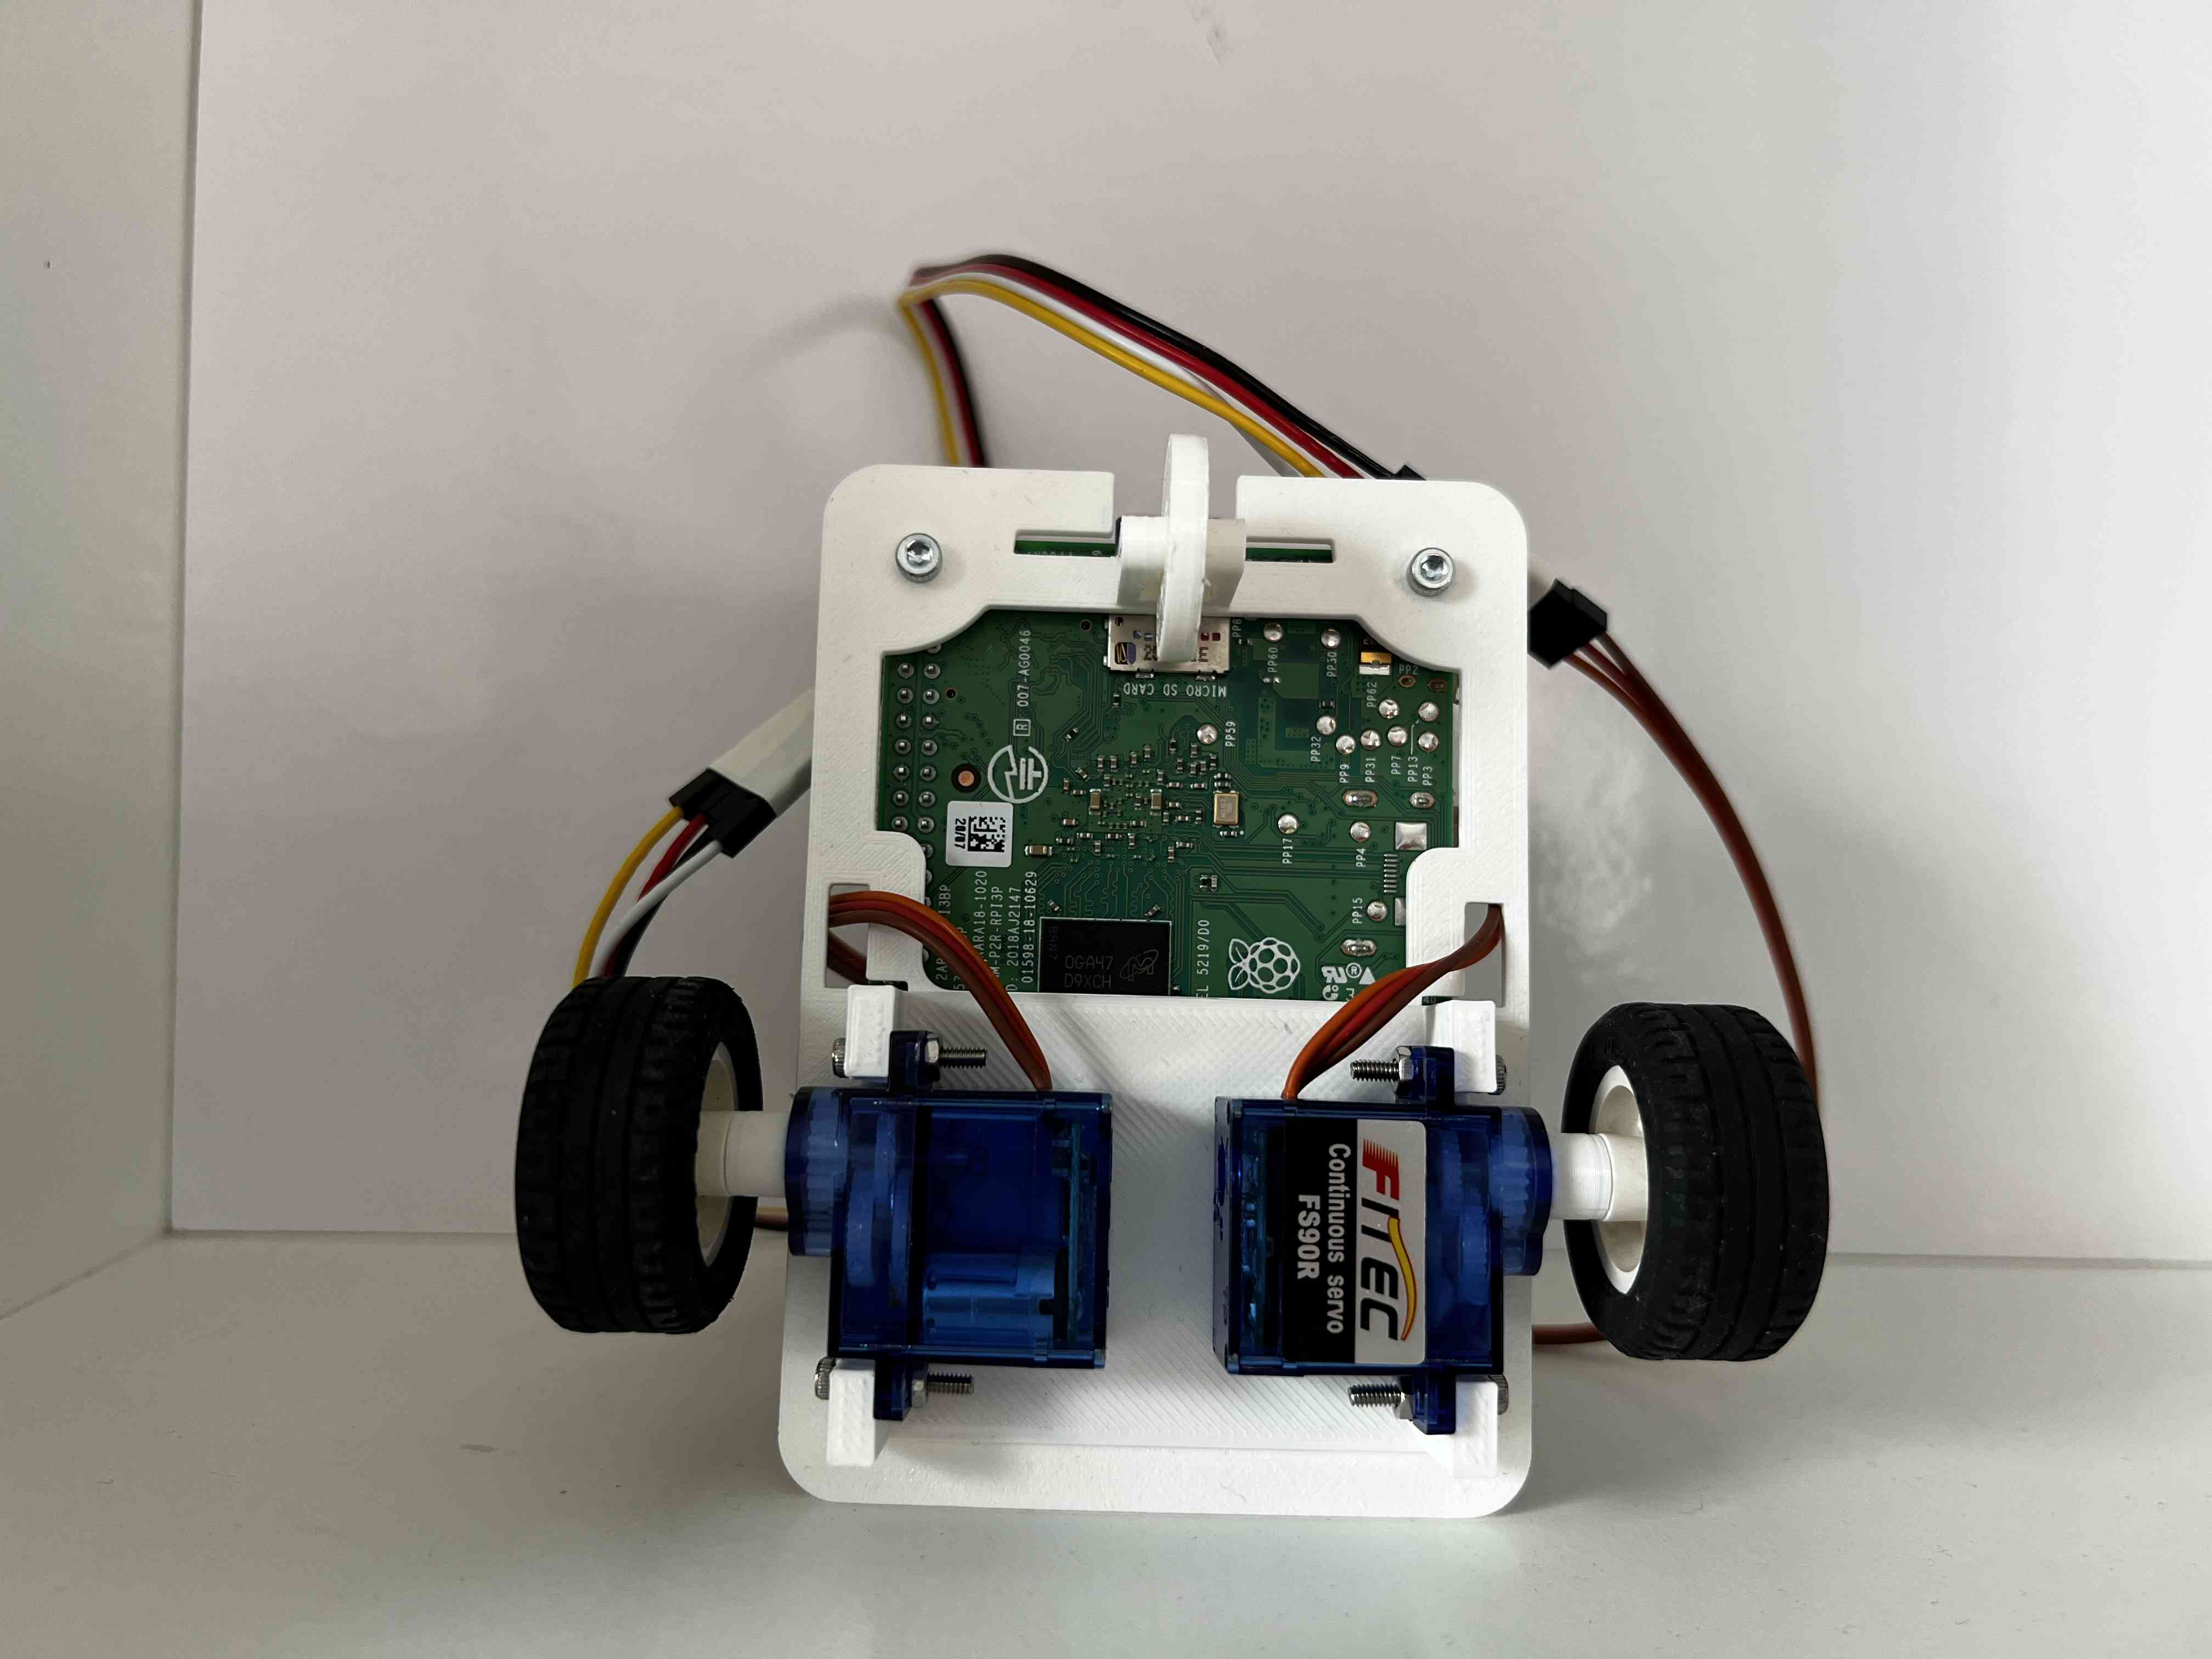
\includegraphics[width=\textwidth]{robot1.jpg}
    \caption{Ansicht von unten}
  \end{subfigure}
  \hspace{1cm}
  \begin{subfigure}[b]{0.45\textwidth}
    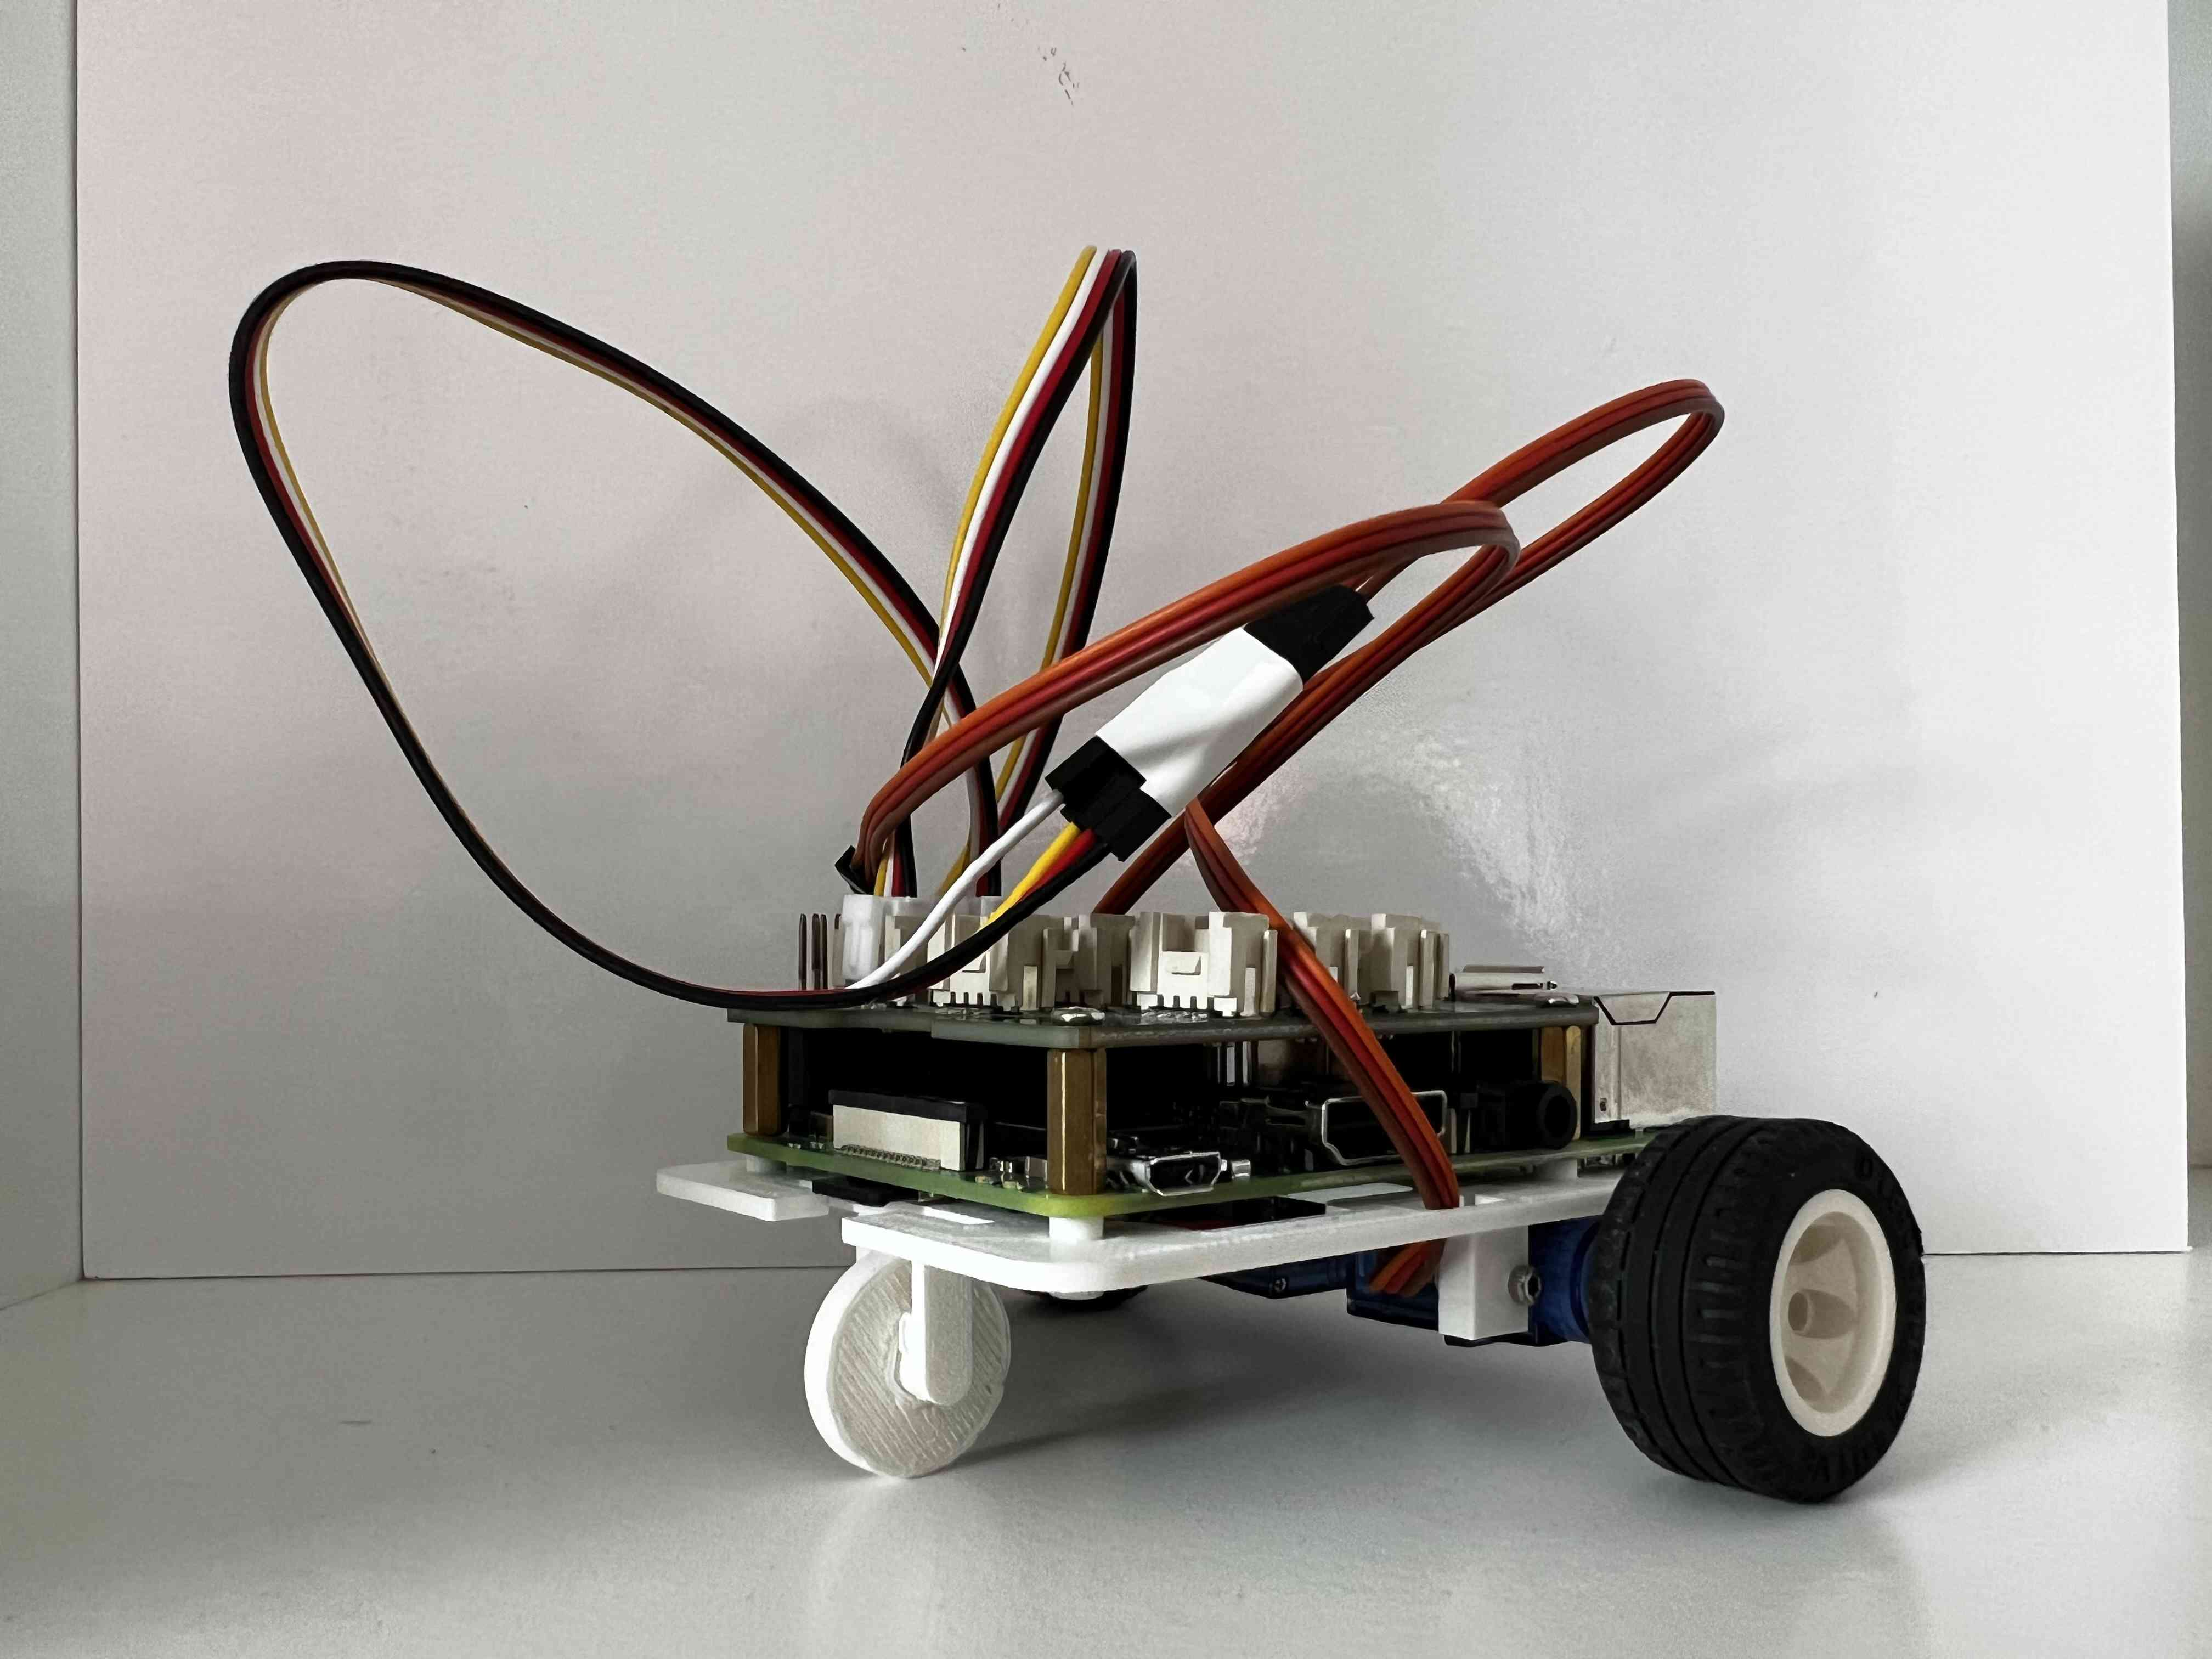
\includegraphics[width=\textwidth]{robot2.jpg}
    \caption{Seitenansicht}
  \end{subfigure}
  \caption{Zusammengebauter Roboter \label{fig:fertiger-roboter}}
\end{figure}

\section{Funktionsweise im Überblick}
Im Folgenden soll eine gesamtheitliche Übersicht geschaffen werden, anhand der die Funktionsweise und Abläufe des Roboters deutlich werden. Die Grundvoraussetzung für die Kommunikation mit dem Roboter ist, dass sich das Gerät, auf dem der Schwarmintelligenz-Algorithmus einen Pfad berechnet und daraus die Instruktionen für den Roboter erstellt, im gleichen Netzwerk angesiedelt sind. Die Kommunikation zwischen den Geräten erfolgt über das Protokoll \textit{HTTP}. Zu Beginn muss an den in \autoref{fig:apidocs} dargestellten Endpunkt \textit{/uploadfile/} eine \textit{JSON}-Datei mit den Instruktionen für den Roboter gesendet werden. Der Aufbau muss wie in \autoref{lst:instructions-json} dargestellt vorliegen. Wenn diese Datei erfolgreich an den Endpunkt des Raspberry Pi übertragen wurde, kann der Roboter gestartet werden. Dies erfolgt über den Endpunkt \textit{/start/}, der im Anschluss der Übertragung aufgerufen werden muss. Nach Aufruf dieses Endpunkts wird auf dem Roboter die zuvor übertragene \textit{JSON}-Datei geladen und anschließend die vorhandenen Instruktionen der Reihenfolge nach durch eine Übersetzungsfunktion ausgeführt. Der vollständige Code zur Ausführung der Instruktionen ist in \autoref{lst:driving_logic} dargestellt. Jeder der Endpunkte gibt eine Rückmeldung, ob die jeweilige Aktion erfolgreich war. 

\inputminted{json}{{assets/code/instructions.json}}
\vspace*{-3mm}
\label{lst:instructions-json}
\captionof{listing}{JSON Instructions}
\vspace*{3mm}

Soll ein neuer Fahrvorgang gestartet werden, muss der Anwender eine neue Datei mit Instruktionen an den Endpunkt senden. Dieser Vorgang ersetzt die zuvor eventuell bereits vorhandene Datei und ermöglicht einen neuen Durchlauf. Der Roboter kann jederzeit über den Endpunkt \textit{/stop/} gestoppt werden.

\section{Probleme bei der Umsetzung}
Im Folgenden sollen Probleme aufgezeigt werden, die bei der Umsetzung, sowohl bei der Konzeption als auch bei der Implementierung, aufgetreten sind. Diese Probleme wurden in der Praxis gelöst und sollen nun in diesem Kapitel erläutert werden.
Damit eine mobile Anwendung des Roboters möglich ist, ist eine Spannungsversorgung mittels eines Akkus notwendig. Der Raspberry Pi 3B+ benötigt eine Versorgungsspannung von 5V, die  über den Micro-USB-Anschluss bereitgestellt werden kann \cite{raspberrypi-docs}. Optimalerweise wird für den Betrieb der Motoren weiterhin eine weitere externe Spanungsquelle verwendet. Diese steht im Rahmen der studentischen Arbeit jedoch nicht zur Verfügung und konnte nicht durch das Inventar der Lehrstätte zur Verfügung gestellt werden. Daher wurde der Rasperry Pi ausschließlich über den Micro-USB-Anschluss mit Strom versorgt, was die Mobilität aufgrund des angeschlossenen Kabels stark einschränkt. 
Bei den vorerst verwendeten Motoren handelt es sich um Motoren, die für den Einsatz in Modellbauanwendungen konzipiert wurden. Hierbei stellte sich zu einem späteren Zeitpunkt der Nachteil heraus, dass diese Motoren nur einen Drehradius von 180° besitzen. Dieser ist für die Bewegung des Roboters nicht ausreichend. Daher wurde ein neuer Motor mit einem Drehradius von 360° verwendet, mit dem die Bewegung des Roboters nun möglich ist.
Weiterhin stellten sich bei der Ansteuerung der Motoren zusätzliche Probleme heraus. Die Ansteuerung der an die GPIO-Pins des Rapsberry angeschlossenen Motoren erfolgt über die Anpassung der \textit{PWM}-Frequenz. Die PWM-Frequenz wird hierbei über die Bibliothek \textit{pigpio} eingestellt. Jedoch stellte sich heraus, dass die Anpassung der PWM-Frequenz nicht zuverlässig funktioniert. Durch die Anpassung sollte es normalerweise möglich sein, die Geschwindigkeit der Motoren zu steuern. Mit der Anpassung war es jedoch lediglich möglich, die Richtung der Drehung der Motoren anzupassen, weswegen eine Anpassung der Fahrgeschwindigkeit des Roboters nicht möglich war. Dies hatte weiterhin zur Folge, dass eine Rechts- sowie Linksdrehung des Roboters nicht während dem Fahren erfolgen kann. Deshalb werden Instruktionen zur Navigation des Rechts- und Linksfahrens nur während des Stillstands des Roboters ausgeführt und Anweisungen hierfür werden inkrementell verarbeitet.
\chapter{Fazit}
% LTeX: language=de-DE
\section{Zusammenfassung}

Für die Umsetzung des Vorhabens wurden drei Konzepte erläutert, miteinander verglichen und anschließend das passendste Konzept anhand von Kriterien ausgewählt.Dabei wurden Faktoren wie die verfügbare Hardware und vorhandene Kenntnisse berücksichtigt. Besonderes Augenmerk wurde auf die Kommunikation zwischen den einzelnen Komponenten gelegt, wobei Aspekte wie Sicherheit, Authentifizierung und Validierung von Daten einbezogen wurden. Hierbei wurde eine Ansteuerung mittels einer REST API gewählt. Damit hierdurch übertragene Daten korrekt verarbeitet werden können, wurde eine Funktion zur Übersetzung von Instruktionen für die Anwendung auf dem Einplatinencomputer implementiert und integriert. Schließlich wurden die Ergebnisse der Planung mit den Hardware-Komponenten vereint, eine geeignete Plattform für den Roboter konstruiert und alles in einem Prototypen zusammengeführt.

\section{Ausblick}
% LTeX: language=de-DE
\appendix
\chapter{Code Darstellungen}
\label{sec:code-darstellungen}

\inputminted{python}{{assets/code/main-api.py}}
\vspace*{-3mm}
\captionof{listing}{API\label{lst:api}}
\vspace*{3mm}

\inputminted{python}{{assets/code/driving_logic.py}}
\vspace*{-3mm}
\captionof{listing}{Driving Logic\label{lst:driving_logic}}
\vspace*{3mm}
>>>>>>> master
\printbibliography
\end{document}
%